\chapter{Connectedly Communicating LTN}

\section{Introduction}

In the previous chapter we considered a \emph{bounded-drift} property for an LTN, similar to the notion considered in~\cite{DBLP:conf/concur/HerbreteauSW22} for networks of timed automata. An LTN is said to have drift bounded by $K$ if in every behaviour, the local-time delays can be \emph{tightened} so that the drift between the local-times of every pair of processes is always bounded by a constant $K$. As we showed in the previous chapter, this property makes reachability decidable by enabling the construction of a region automaton for the set of untimed behaviours.

In this chapter, we identify a structural fragment of LTNs where bounded drift holds automatically. We call this fragment \emph{connectedly-communicating} negotiations.

\subsection{The Connectedly-Communicating Fragment}

As we have seen in previous chapters, local-timed negotiations (LTNs) sit between two well-behaved extremes: on the one hand, fully synchronizing LTNs behave essentially like a single global clock; on the other hand, synchronization-free LTNs behave like independent local clocks. The difficulty begins exactly when we \emph{mix} local time elapse with occasional time-synchronizing negotiations. Then one process can wait for a long time, later force another process to catch up at a synchronizing node, and thereby transport large time gaps across the system. This is precisely the mechanism behind the undecidability phenomena established earlier.

This chapter isolates a robust \emph{structural} reason why such transport of time gaps can be controlled. The key intuition is:
\begin{quote}
If, in every cycle of the control structure, time-synchronizations connect all agents (directly or through a chain), then no agent can accumulate unbounded local time without repeatedly synchronizing it back into the rest of the system.
\end{quote}

We formalize this intuition through the notion of \emph{connectedly-communicating} LTNs and prove that this structural condition forces bounded drift.

\paragraph*{Main result.}
Our main theorem shows that connected communication implies a uniform drift bound.

\begin{theorem}[Informal statement]
Every connectedly-communicating local-timed negotiation is drift-bounded. More precisely, if $\Nn$ is connectedly-communicating, then every behaviour of $\Nn$ can be tightened so that the drift between any two processes is bounded by
\[
O(|N|\cdot |P|^3 \cdot (M+1)),
\]
where $N$ is the set of negotiation nodes, $P$ is the set of processes, and $M$ is the largest timing constant appearing in the guards.
\end{theorem}

Combined with the region-style construction from the previous chapter, this immediately yields the following consequence.

\begin{corollary}[Informal statement]
Reachability is decidable for connectedly-communicating LTNs.
\end{corollary}

Thus, the chapter identifies a natural structural fragment of LTNs that still allows partial local-time evolution, but rules out the unbounded drift patterns responsible for undecidability.

\paragraph*{Two proof layers: local tightening, then global boundedness.}
The proof decomposes into two conceptually separate layers:
\begin{enumerate}
    \item \textbf{Tightening (local normal form).} Every run can be transformed into a run in which no unnecessary waiting above $M{+}1$ remains, except what is forced by time-synchronizations. This step is purely semantic and does not use connected communication.
    \item \textbf{Bounded drift (global consequence of connectivity).} For connectedly-communicating LTNs, timestamps in a tightened run cannot diverge arbitrarily: connectivity forces the effect of synchronizations to propagate across all processes within a bounded amount of control progress.
\end{enumerate}

\paragraph*{Related work.}
The idea that connected communication restores decidability is inspired by two classical results:
\begin{enumerate}
    \item Alur and Yannakakis's work on hierarchical message sequence graphs~\cite{DBLP:conf/concur/AlurY99}, where a related connectedness requirement yields decidability of emptiness, and
    \item Madhusudan, Thiagarajan, and Yang's work on distributed controller synthesis~\cite{DBLP:conf/fsttcs/MadhusudanTY05}, where a suitable connectedness condition again rescues decidability from an otherwise undecidable setting.
\end{enumerate}

Our setting differs somewhat from~\cite{DBLP:conf/fsttcs/MadhusudanTY05}, where the requirement is in fact weaker: roughly speaking, if process $p$ never hears from $q$ (directly or indirectly) along a cycle, then $p$ and $q$ never synchronize again in the future. We discuss this weaker variant in Section~\ref{sec:conclusion}.

The notion of drift has also been studied extensively for networks of timed automata in~\cite{DBLP:conf/lics/0001HSW22,DBLP:conf/concur/HerbreteauSW22}. In that setting, local-time semantics supports more efficient symbolic verification by avoiding one dimension of exponential blowup caused by interleaving independent actions. Bounded drift then provides simulation arguments ensuring finiteness of zone-based exploration.

\paragraph*{Organization of the chapter.}
Section~\ref{sec:prelims} recalls the definition of local-timed negotiations and introduces our trace-based view of behaviours, which will be essential for the technical development. Section~\ref{sec:bounded} recalls the drift-bounded framework from the previous chapter and the reachability consequences that we will use here. Our main technical contribution begins in Section~\ref{sec:connected}, where we prove that connectedly-communicating LTNs have bounded drift. The proof proceeds in two main steps: in (Section~\ref{sec:tighten}) we describe tightening, i.e., how to systematically reduce time delays in any run while preserving validity; and in (Section~\ref{sec:cc-ltn-bounded}) we prove that tight runs of connectedly-communicating LTNs have uniformly bounded drift.
Section~\ref{sec:conclusion} concludes the chapter and discusses extensions and future directions.

%-----------------------------------------------------------------------------------------------------

\section{Understanding Connectedly Communicating LTNs Through Examples}
\label{sec:prelims}

Before turning to the formal development, we discuss a small family of examples
that illustrates the structural idea behind connected communication. The point of
these examples is not to analyze all timed behaviours in full detail, but to show
how the pattern of \emph{time-synchronizing contacts along loops of the marking graph}
controls the possibility of unbounded drift.

Figure~\ref{fig:three-in-one} shows three closely related LTNs with the same
overall control structure, but with different synchronization patterns. These
differences are not yet fully visible at the level of the LTN itself. They become
clearer when we pass to loops in the untimed marking graph and then abstract each
such loop to a graph on agents that records which pairs of agents synchronize
together along that loop. Figures~\ref{fig:marking-graphs}
and~\ref{fig:comm-graphs} make this viewpoint explicit, while
Figure~\ref{fig:multiple-iterations} illustrates that, even in the
connectedly-communicating setting, propagation of timing information may require
several iterations.

\begin{figure}[t]
\centering
\begin{minipage}{0.5\textwidth}
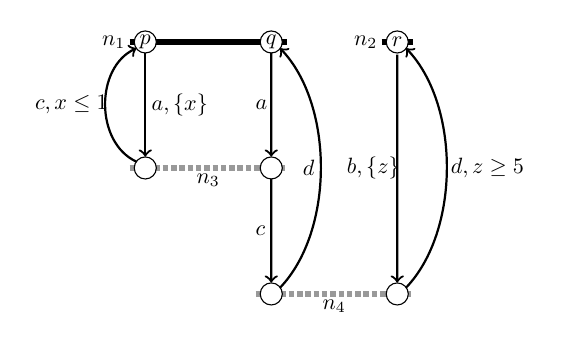
\begin{tikzpicture}[scale=0.8, every node/.style={transform shape}]

\begin{scope}[line width=2pt]
\draw (-0.25,0) -- (2.25,0);
\draw (3.75,0) -- (4.25,0);
\draw [opacity=0.4, densely dotted] (-0.25,-2) -- (2.25,-2);
\draw [opacity=0.4, densely dotted] (1.75,-4) -- (4.25,-4);
\end{scope}

\filldraw [fill=white]  (0,0)  circle (1.75mm) node (p1) {$p$};
\filldraw [fill=white]  (2,0)  circle (1.75mm) node (q1) {$q$};
\filldraw [fill=white]  (4,0)  circle (1.75mm) node (r2) {$r$};
\filldraw [fill=white]  (0,-2)  circle (1.75mm) node (p3) {};
\filldraw [fill=white]  (2,-2)  circle (1.75mm) node (q3) {};
\filldraw [fill=white]  (2,-4)  circle (1.75mm) node (q4) {};
\filldraw [fill=white]  (4,-4)  circle (1.75mm) node (r4) {};

\node at (-0.5,0) {$n_1$};
\node at (3.5,0) {$n_2$};
\node at (1,-2.2) {$n_3$};
\node at (3,-4.2) {$n_4$};
\node at (0.6,-1) [text width=1cm] {$a, \{x\}$};
\node at (2.25,-1) [text width=1cm] {$a$};
\node at (3.7,-2) [text width=1cm] {$b, \{z\}$};
\node at (2.25,-3) [text width=1cm] {$c$};
\node at (-1,-1) [text width=1.5cm] {$c, x \leq 1$};
\node at (3,-2) [text width=1cm] {$d$};
\node at (5.6,-2) [text width=1.5cm] {$d, z \geq 5$};

\begin{scope}[thick,->]
\draw (p1) + (0, -0.17) -- (0,-1.82);
\draw (q1) + (0, -0.17) -- (2,-1.82);
\draw (q3) + (0, -0.17) -- (2,-3.82);
\draw (r2) -- (4,-3.82);
\draw (-0.14,-1.9) .. controls (-0.8,-1.6) and (-0.8,-0.4) .. (-0.14,-0.1);
\draw (2.14,-3.9) .. controls (3,-3) and (3,-1) .. (2.14,-0.1);
\draw (4.14,-3.9) .. controls (5,-3) and (5,-1) .. (4.14,-0.1);
\end{scope}

\end{tikzpicture}
\end{minipage}
\begin{minipage}{0.5\textwidth}
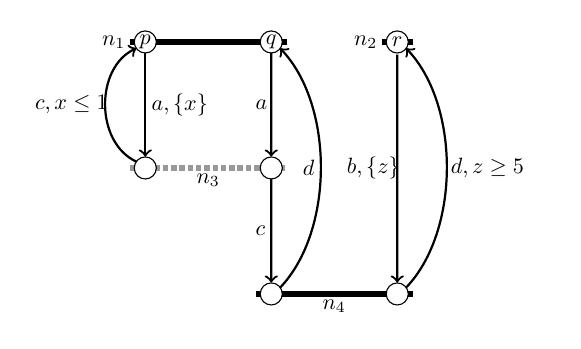
\begin{tikzpicture}[scale=0.8, every node/.style={transform shape}]

\begin{scope}[line width=2pt]
\draw (-0.25,0) -- (2.25,0);
\draw (3.75,0) -- (4.25,0);
\draw [opacity=0.4, densely dotted] (-0.25,-2) -- (2.25,-2);
\draw (1.75,-4) -- (4.25,-4);
\end{scope}

\filldraw [fill=white]  (0,0)  circle (1.75mm) node (p1) {$p$};
\filldraw [fill=white]  (2,0)  circle (1.75mm) node (q1) {$q$};
\filldraw [fill=white]  (4,0)  circle (1.75mm) node (r2) {$r$};
\filldraw [fill=white]  (0,-2)  circle (1.75mm) node (p3) {};
\filldraw [fill=white]  (2,-2)  circle (1.75mm) node (q3) {};
\filldraw [fill=white]  (2,-4)  circle (1.75mm) node (q4) {};
\filldraw [fill=white]  (4,-4)  circle (1.75mm) node (r4) {};

\node at (-0.5,0) {$n_1$};
\node at (3.5,0) {$n_2$};
\node at (1,-2.2) {$n_3$};
\node at (3,-4.2) {$n_4$};
\node at (0.6,-1) [text width=1cm] {$a, \{x\}$};
\node at (2.25,-1) [text width=1cm] {$a$};
\node at (3.7,-2) [text width=1cm] {$b, \{z\}$};
\node at (2.25,-3) [text width=1cm] {$c$};
\node at (-1,-1) [text width=1.5cm] {$c, x \leq 1$};
\node at (3,-2) [text width=1cm] {$d$};
\node at (5.6,-2) [text width=1.5cm] {$d, z \geq 5$};

\begin{scope}[thick,->]
\draw (p1) + (0, -0.17) -- (0,-1.82);
\draw (q1) + (0, -0.17) -- (2,-1.82);
\draw (q3) + (0, -0.17) -- (2,-3.82);
\draw (r2) -- (4,-3.82);
\draw (-0.14,-1.9) .. controls (-0.8,-1.6) and (-0.8,-0.4) .. (-0.14,-0.1);
\draw (2.14,-3.9) .. controls (3,-3) and (3,-1) .. (2.14,-0.1);
\draw (4.14,-3.9) .. controls (5,-3) and (5,-1) .. (4.14,-0.1);
\end{scope}

\end{tikzpicture}
\end{minipage}
\begin{minipage}{0.5\textwidth}
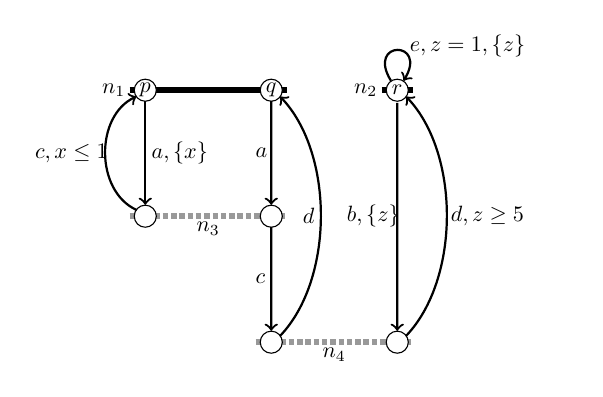
\begin{tikzpicture}[scale=0.8, every node/.style={transform shape}]

\begin{scope}[line width=2pt]
\draw (-0.25,0) -- (2.25,0);
\draw (3.75,0) -- (4.25,0);
\draw [opacity=0.4, densely dotted] (-0.25,-2) -- (2.25,-2);
\draw [opacity=0.4, densely dotted] (1.75,-4) -- (4.25,-4);
\end{scope}

\filldraw [fill=white]  (0,0)  circle (1.75mm) node (p1) {$p$};
\filldraw [fill=white]  (2,0)  circle (1.75mm) node (q1) {$q$};
\filldraw [fill=white]  (4,0)  circle (1.75mm) node (r2) {$r$};
\filldraw [fill=white]  (0,-2)  circle (1.75mm) node (p3) {};
\filldraw [fill=white]  (2,-2)  circle (1.75mm) node (q3) {};
\filldraw [fill=white]  (2,-4)  circle (1.75mm) node (q4) {};
\filldraw [fill=white]  (4,-4)  circle (1.75mm) node (r4) {};

\node at (-0.5,0) {$n_1$};
\node at (3.5,0) {$n_2$};
\node at (1,-2.2) {$n_3$};
\node at (3,-4.2) {$n_4$};
\node at (0.6,-1) [text width=1cm] {$a, \{x\}$};
\node at (2.25,-1) [text width=1cm] {$a$};
\node at (3.7,-2) [text width=1cm] {$b, \{z\}$};
\node at (2.25,-3) [text width=1cm] {$c$};
\node at (-1,-1) [text width=1.5cm] {$c, x \leq 1$};
\node at (3,-2) [text width=1cm] {$d$};
\node at (5.6,-2) [text width=1.5cm] {$d, z \geq 5$};
\node at (5.45,0.7) [text width=2.5cm] {$e, z=1, \{z\}$};

\begin{scope}[thick,->]
\draw (p1) + (0, -0.17) -- (0,-1.82);
\draw (q1) + (0, -0.17) -- (2,-1.82);
\draw (q3) + (0, -0.17) -- (2,-3.82);
\draw (r2) -- (4,-3.82);
\draw (-0.14,-1.9) .. controls (-0.8,-1.6) and (-0.8,-0.4) .. (-0.14,-0.1);
\draw (2.14,-3.9) .. controls (3,-3) and (3,-1) .. (2.14,-0.1);
\draw (4.14,-3.9) .. controls (5,-3) and (5,-1) .. (4.14,-0.1);
\draw (3.9,0.15) .. controls (3.5,0.8) and (4.5,0.8) .. (4.1,0.15);
\end{scope}

\end{tikzpicture}
\end{minipage}
\caption{Three variations of LTNs illustrating different synchronization patterns.
(a) Connectedly communicating; (b) not connectedly communicating because one
synchronizing link is missing; (c) not connectedly communicating because of an
isolated local loop, leading to unbounded drift.}
\label{fig:three-in-one}
\end{figure}

\begin{example}\label{eg:three-in-one}
Let
\[
C=(\{n_1\},\{n_1\},\{n_2\})
\]
be the marking in which the three agents \(p,q,r\) are ready at \(n_1,n_1,n_2\),
respectively. For each of the three LTNs in Figure~\ref{fig:three-in-one},
Figure~\ref{fig:marking-graphs} shows a representative loop from \(C\) back to
\(C\) in the untimed marking graph \(\mg(\nuntime)\), and
Figure~\ref{fig:comm-graphs} shows the corresponding communication graph.

\begin{figure}[t]
\centering

\begin{minipage}{0.32\textwidth}
\centering
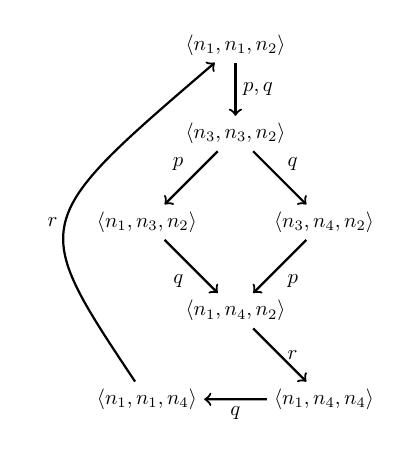
\begin{tikzpicture}[scale=0.75, every node/.style={transform shape}]
    \node (s0) at (0, 0) {$\langle n_1, n_1, n_2 \rangle$};
    \node (s1) at (0, -1.5) {$\langle n_3, n_3, n_2 \rangle$};
    \node (s2) at (-1.5, -3) {$\langle n_1, n_3, n_2 \rangle$};
    \node (s3) at (1.5, -3) {$\langle n_3, n_4, n_2 \rangle$};
    \node (s4) at (0, -4.5) {$\langle n_1, n_4, n_2 \rangle$};
    \node (s5) at (1.5, -6) {$\langle n_1, n_4, n_4 \rangle$};
    \node (s6) at (-1.5, -6) {$\langle n_1, n_1, n_4 \rangle$};

    \draw[->, thick] (s0) -- (s1) node[midway, right] {$p,q$};
    \draw[->, thick] (s1) -- (s2) node[midway, above left] {$p$};
    \draw[->, thick] (s1) -- (s3) node[midway, above right] {$q$};
    \draw[->, thick] (s2) -- (s4) node[midway, below left] {$q$};
    \draw[->, thick] (s3) -- (s4) node[midway, below right] {$p$};
    \draw[->, thick] (s4) -- (s5) node[midway, right] {$r$};
    \draw[->, thick] (s5) -- (s6) node[midway, below] {$q$};
    \draw[->, thick] (s6) .. controls (-3.5, -3) .. (s0) node[midway, left] {$r$};
\end{tikzpicture}
\subcaption*{(a) A loop whose synchronizing contacts connect all agents}
\end{minipage}
\hfill
\begin{minipage}{0.32\textwidth}
\centering
\begin{tikzpicture}[scale=0.75, every node/.style={transform shape}]
    \node (s0) at (0, 0) {$\langle n_1, n_1, n_2 \rangle$};
    \node (s1) at (0, -1.5) {$\langle n_3, n_3, n_2 \rangle$};
    \node (s2) at (-1.5, -3) {$\langle n_1, n_3, n_2 \rangle$};
    \node (s3) at (1.5, -3) {$\langle n_3, n_4, n_2 \rangle$};
    \node (s4) at (0, -4.5) {$\langle n_1, n_4, n_4 \rangle$};
    \node (s5) at (0, -6) {$\langle n_1, n_1, n_2 \rangle$};

    \draw[->, thick] (s0) -- (s1) node[midway, right] {$p,q$};
    \draw[->, thick] (s1) -- (s2) node[midway, above left] {$p$};
    \draw[->, thick] (s1) -- (s3) node[midway, above right] {$q$};
    \draw[->, thick] (s2) -- (s4) node[midway, below left] {$q,r$};
    \draw[->, thick] (s3) -- (s4) node[midway, below right] {$p,r$};
    \draw[->, thick] (s4) -- (s5) node[midway, right] {$q,r$};
    \node[draw=red, dashed, inner sep=2mm, fit=(s4)] {};
\end{tikzpicture}
\subcaption*{(b) A disconnected loop}
\end{minipage}
\hfill
\begin{minipage}{0.32\textwidth}
\centering
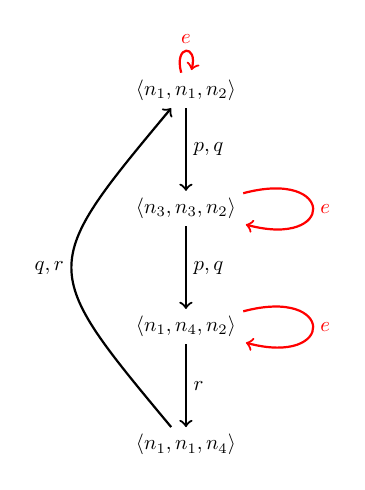
\begin{tikzpicture}[scale=0.75, every node/.style={transform shape}]
    \node (s0) at (0, 0) {$\langle n_1, n_1, n_2 \rangle$};
    \node (s1) at (0, -2) {$\langle n_3, n_3, n_2 \rangle$};
    \node (s4) at (0, -4) {$\langle n_1, n_4, n_2 \rangle$};
    \node (s6) at (0, -6) {$\langle n_1, n_1, n_4 \rangle$};

    \draw[->, thick] (s0) -- (s1) node[midway, right] {$p,q$};
    \draw[->, thick] (s1) -- (s4) node[midway, right] {$p,q$};
    \draw[->, thick] (s4) -- (s6) node[midway, right] {$r$};
    \draw[->, thick] (s6) .. controls (-2.5, -3) .. (s0) node[midway, left] {$q,r$};

    \path[->, thick, red] (s0) edge [loop above] node {$e$} (s0);
    \path[->, thick, red] (s1) edge [loop right] node {$e$} (s1);
    \path[->, thick, red] (s4) edge [loop right] node {$e$} (s4);
\end{tikzpicture}
\subcaption*{(c) An isolated local loop}
\end{minipage}

\caption{Representative loops in the untimed marking graphs \(\mg(\nuntime)\) for
the three variants. These loops will be used to extract the communication graphs
of Figure~\ref{fig:comm-graphs} by recording which agents synchronize together
along each loop.}
\label{fig:marking-graphs}
\end{figure}

To analyze whether timing information can propagate through a cyclic behaviour, we
proceed in two steps. First, we look at a loop in the untimed marking graph
\(\mg(\nuntime)\), as illustrated in Figure~\ref{fig:marking-graphs}. Such a loop
records which local moves can occur cyclically from a given marking, but it still
contains more information than we need for connected communication.

From this loop, we then extract a simpler graph whose vertices are the agents.
We put an edge between two agents \(p\) and \(q\) whenever some
time-synchronizing node appearing on the chosen loop has both \(p\) and \(q\) in
its domain. In other words, the communication graph forgets the intermediate
markings and remembers only which agents are forced to time-synchronize together
somewhere along that loop. Figure~\ref{fig:comm-graphs} shows the communication
graphs obtained from the loops of Figure~\ref{fig:marking-graphs}.

\begin{figure}[ht]
\centering

\begin{minipage}{0.32\textwidth}
\centering
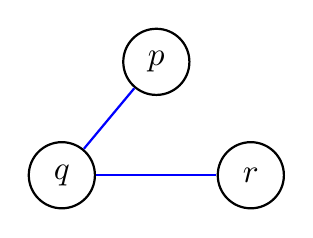
\begin{tikzpicture}[scale=1.2, every node/.style={transform shape}]
    \node[circle, draw, thick, minimum size=7mm] (p) at (0, 1.2) {$p$};
    \node[circle, draw, thick, minimum size=7mm] (q) at (-1, 0) {$q$};
    \node[circle, draw, thick, minimum size=7mm] (r) at (1, 0) {$r$};

    \draw[thick, blue] (p) -- (q);
    \draw[thick, blue] (q) -- (r);
\end{tikzpicture}
\subcaption*{(a) Connected}
\end{minipage}
\hfill
\begin{minipage}{0.32\textwidth}
\centering
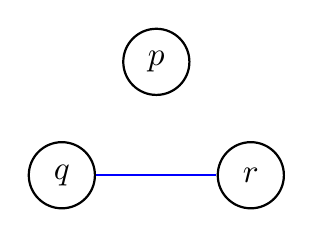
\begin{tikzpicture}[scale=1.2, every node/.style={transform shape}]
    \node[circle, draw, thick, minimum size=7mm] (p) at (0, 1.2) {$p$};
    \node[circle, draw, thick, minimum size=7mm] (q) at (-1, 0) {$q$};
    \node[circle, draw, thick, minimum size=7mm] (r) at (1, 0) {$r$};

    \draw[thick, blue] (q) -- (r);
\end{tikzpicture}
\subcaption*{(b) Disconnected on the chosen loop}
\end{minipage}
\hfill
\begin{minipage}{0.32\textwidth}
\centering
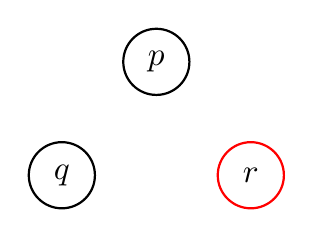
\begin{tikzpicture}[scale=1.2, every node/.style={transform shape}]
    \node[circle, draw, thick, minimum size=7mm] (p) at (0, 1.2) {$p$};
    \node[circle, draw, thick, minimum size=7mm] (q) at (-1, 0) {$q$};
    \node[circle, draw, thick, minimum size=7mm, draw=red] (r) at (1, 0) {$r$};
\end{tikzpicture}
\subcaption*{(c) Totally disconnected}
\end{minipage}

\caption{Communication graphs extracted from the loops shown in
Figure~\ref{fig:marking-graphs}. The vertices are the agents, and two agents are
connected whenever they participate together in some time-synchronizing node
occurring on the corresponding loop.}
\label{fig:comm-graphs}
\end{figure}

 Figure~\ref{fig:comm-graphs} extracts, from the representative loops of
Figure~\ref{fig:marking-graphs}, the corresponding communication graphs. The
vertices are the participating agents, and two agents are joined by an edge
whenever they occur together in some time-synchronizing node along the chosen
loop. In (a), the graph is connected, which is the structural pattern underlying
the connectedly-communicating property. In (b), the graph is disconnected for the
chosen loop, showing that loop-level connectedness fails here. In (c), agent
\(r\) is completely isolated, reflecting the presence of a purely local loop and
the resulting possibility of unbounded drift.

\paragraph{Example (a): connectedly communicating.}
Consider the loop from \(C\) back to \(C\) obtained by executing the outcomes
\(a,b,d,c\). Along this loop, the time-synchronizing nodes are
\[
n_3 \text{ with participants } \{p,q\},
\qquad
n_4 \text{ with participants } \{q,r\}.
\]
Hence the induced communication graph has edges \((p,q)\) and \((q,r)\), and is
therefore the connected path
\[
p-q-r.
\]
This is exactly the pattern required by connected communication.

For intuition, consider one traversal of the cycle from the marking
\((n_1,n_1,n_2)\). At \(n_1\), agents \(p\) and \(q\) execute \(a\). Since
\(n_1\) is not time-synchronizing, they may do so at different local times. The
reset of \(x\) at \(a\), together with the guard \(x\le 1\) at the
time-synchronizing node \(n_3\), forces \(p\) and \(q\) to meet again within one
time unit from \(p\)'s reset.

Meanwhile, agent \(r\) traverses the loop through \(n_2\) and \(n_4\), where the
reset of \(z\) and the guard \(z\ge 5\) force each iteration to take at least
\(5\) time units. When \(q\) synchronizes with \(r\) at \(n_4\), this timing
constraint is transferred to \(q\), and later propagated from \(q\) back to \(p\)
through their own synchronizations. Thus timing information flows through the
chain \(r \leftrightarrow q \leftrightarrow p\), which is the key reason drift
remains bounded.

\paragraph{Example (b): a disconnected loop.}
Now suppose that \(n_4\) is no longer time-synchronizing, as in
Figure~\ref{fig:three-in-one}(b). Then on the analogous loop the only
time-synchronizing node is \(n_3\), with participants \(\{p,q\}\). The induced
communication graph therefore contains only the edge \((p,q)\), while \(r\) is
isolated. Thus this example is \emph{not} connectedly communicating.

The reason drift can now blow up is that time accumulated by \(r\) is no longer
forced back into the rest of the system through synchronization. The pair
\((p,q)\) may remain mutually constrained, but \(r\) can move arbitrarily far
away in local time without creating any contradiction.

Thus Example~(b) lies outside the strict connectedly-communicating fragment. A
weaker relaxation of this condition will be introduced later in
Section~\ref{sec:weaker-connected-comm}.

%What this shows is that one disconnected loop is enough to destroy the direct argument used for Example~(a): timing information accumulated by \(r\) does not have to propagate back to \(p\) through synchronizing contacts on that loop. Nevertheless, the marking-graph picture in Figure~\ref{fig:marking-graphs}(b) suggests a subtler possibility: even though the chosen loop is disconnected, the global structure may still force the run through a later bottleneck where the separated parts are re-coordinated. This is precisely the phenomenon captured by the weaker split-based variant developed in Section~\ref{sec:weaker-connected-comm}. Thus Example~(b) should be read here as a motivation for that later refinement, rather than as part of the strict connectedly-communicating fragment.

\paragraph{Example (c): an isolated local loop and unbounded drift.}
Finally, Figure~\ref{fig:three-in-one}(c) adds a self-loop \(e\) at \(n_2\) for
agent \(r\). Consider the one-step loop
\[
C \xrightarrow{e} C.
\]
No time-synchronizing node appears on this loop. Hence the communication graph
has vertex set \(\{p,q,r\}\) and no edges at all, so it is totally disconnected.

Here the possibility of unbounded drift is immediate: agent \(r\) can iterate the
local loop \(e\) arbitrarily many times while \(p\) and \(q\) remain where they
are. Thus \(r\) can accumulate arbitrarily large local time without any
synchronizing contact. This is the kind of behaviour that later makes region-like
arguments fail.\\

The previous examples show when loop-level connectedness holds or fails. Even in
the positive case, however, timing information need not propagate across all
processes in a single step.

\begin{figure}[t]
\centering
\begin{tikzpicture}[
    >=Latex,
    thick,
    x=1cm,y=1cm,
    every node/.style={font=\small},
    atom/.style={draw,circle,minimum size=6mm,inner sep=0pt},
    aux/.style={circle,fill,inner sep=1.2pt},
    dep/.style={dashed},
    outcome/.style={font=\scriptsize,fill=white,inner sep=1pt},
    note/.style={align=left,font=\small}
]

\node[atom] (n1) at (0,2.5) {$1$};
\node[atom] (n2) at (2.7,2.5) {$2$};
\node[atom] (n3) at (4.9,2.5) {$3$};
\node[atom] (n4) at (7.3,2.5) {$4$};
\node[atom] (n5) at (9.5,2.5) {$5$};

\draw (n2) -- (n3);
\draw (n4) -- (n5);

\node[aux] (m1) at (0,0.30) {};
\node[aux] (m2) at (2.7,1.20) {};
\node[aux] (m3) at (2.7,0.00) {};
\node[aux] (m4) at (4.9,1.05) {};
\node[aux] (m5) at (4.9,0.55) {};
\node[aux] (m6) at (7.3,0.50) {};
\node[aux] (m7) at (7.3,-0.10) {};
\node[aux] (m8) at (9.5,-0.10) {};
\node[aux] (m0) at (0.95,-0.05) {};

\draw[->] (n1) -- node[outcome,right] {$a_1$} (m1);
\draw[->] (-0.60,0.35) to[out=110,in=245] node[outcome,left] {$b_1$} (-0.05,2.42);

\draw[->] (n2) -- node[outcome,right] {$a_2$} (m2);
\draw[->] (m2) -- node[outcome,right] {$b_2$} (m3);
\draw[->] (2.00,0.28) to[out=110,in=245] node[outcome,left] {$c_2$} (2.55,2.42);

\draw[->] (n3) -- node[outcome,right] {$a_3$} (m4);
\draw[->] (5.45,0.82) to[out=65,in=300] node[outcome,right] {$b_3$} (5.00,2.42);

\draw[->] (n4) -- node[outcome,right] {$a_4$} (m6);
\draw[->] (m6) -- node[outcome,right] {$b_4$} (m7);
\draw[->] (7.95,0.25) to[out=70,in=295] node[outcome,right] {$c_4$} (7.45,2.42);

\draw[->] (n5) -- node[outcome,right] {$a_5$} (m8);
\draw[->] (10.10,0.25) to[out=70,in=300] node[outcome,right] {$b_5$} (9.65,2.42);

\draw[dep] (m0) -- node[outcome,below] {$d_1$} (m3);
\draw[dep] (m2) -- node[outcome,below] {$d_2$} (m4);
\draw[dep] (m5) -- node[outcome,below] {$d_3$} (m6);
\draw[dep] (m7) -- node[outcome,below] {$d_4$} (m8);

\node[font=\scriptsize] at (0,3.15) {$\mathsf{dom}(n_1)$};
\node[font=\scriptsize] at (2.7,3.15) {$\mathsf{dom}(n_2)$};
\node[font=\scriptsize] at (4.9,3.15) {$\mathsf{dom}(n_3)$};
\node[font=\scriptsize] at (7.3,3.15) {$\mathsf{dom}(n_4)$};
\node[font=\scriptsize] at (9.5,3.15) {$\mathsf{dom}(n_5)$};

\node[note,anchor=west] at (11.0,1.2) {%
It takes at least $2$ iterations\\
for the information of $5$\\
to reach $1$.};

\end{tikzpicture}
\caption{A schematic example showing that timing information need not propagate
to all agents within a single propagation step. In general, the propagation
argument may require up to \(|P|\) iterations; in this example, timing
information originating at node \(5\) reaches node \(1\) only after \(2\)
iterations, through a chain of intermediate dependencies.}
\label{fig:multiple-iterations}
\end{figure}

\paragraph{Iterated propagation of timing information.} Figure~\ref{fig:multiple-iterations} illustrates an important feature of the
propagation argument even in the ordinary connectedly communicating setting.
Connectedness of the communication structure does not mean that timing
information becomes globally available in a single step. Rather, one obtains a
local propagation effect, and this effect must be iterated.

Starting from one process (here, process \(5\)), the timing information first
reaches only those processes that are directly linked to it by the relevant local
dependencies. In the next round, it can propagate further to processes that are
linked to those, and so on. Thus the proof proceeds by repeated closure under
this propagation relation. In general, timing information propagates at most one edge farther in each iteration. Hence the number of iterations needed is bounded by the length of the longest path in the communication graph, and therefore by \(|P|-1\). In the present example, \(2\) iterations are necessary for the influence of process
\(5\) to reach process \(1\).

\paragraph{Takeaway.}
These examples isolate the structural issue behind the chapter. In
Example~(a), the synchronizing contacts that occur on the loop connect all
agents, so timing constraints can propagate throughout the system. In
Example~(b), this loop-level connectedness fails: one agent is no longer tied
back to the others through synchronizing contacts on the loop, and unbounded
drift becomes possible. In Example~(c), the failure is more drastic, since there
is a genuinely isolated local loop, and unbounded drift follows immediately. The
bounded-drift theorem proved later in the chapter shows that the positive pattern
exemplified by (a) is exactly the one that suffices for the main decidability
argument.
\end{example}

%----------------------------------------------------------------------------------------------------------------------

\section{Connectedly communicating LTNs}
\label{sec:connected}

Now we're ready to formally define connectedly-communicating LTNs and prove our main result: that this fragment has bounded drift. We'll build this up in stages, first defining the necessary graph-theoretic concepts, then explaining the tightening procedure, and finally proving the bound.

\subsection{Marking Graphs and Communication Graphs}

To define connectedness, we need to look at two different graphs derived from an LTN.

\paragraph*{The Untimed Negotiation $\nuntime$}

For an LTN $\Nn$, let $\nuntime$ denote the untimed version obtained by structurally removing all clock guards and resets from transitions. This gives us an over-approximation of possible behaviors---if something is impossible in $\nuntime$, it's impossible in $\Nn$, but some behaviors of $\nuntime$ might not be achievable in $\Nn$ due to timing constraints.

\paragraph*{The Marking Graph $\mg(\nuntime)$}

The marking graph captures which nodes agents can be at simultaneously. A \emph{marking} $C$ maps each agent to a set of nodes that agent participates in. 

The vertices of $\mg(\nuntime)$ are all possible markings. There is an edge $C \xra{n} C'$ if node $n$ is enabled at marking $C$ (meaning $n \in C(p)$ for all agents $p$ participating in $n$), and $C'$ is the marking after executing $n$.
The three variants in our running example (Figure~\ref{fig:three-in-one}) provide a useful illustration: For each of the LTNs of our running example (Figure~\ref{fig:three-in-one}), Figure~\ref{fig:marking-graphs} shows the corresponding marking graphs. The marking graphs make explicit the loops on which our connectedness condition will later be imposed.

%This is a finite graph with size at most $2^{|N|} \cdot |P|$ where $|N|$ is the number of nodes in $\Nn$.

\paragraph*{Markings and the size of the marking graph.}
Since we work with $\nuntime$ where outcomes are abstracted away in the edge labels (we write $C \xra{n} C'$ rather than $C \xra{(n,a)} C'$), a marking records, for each agent, \emph{a set of possible current nodes}.
Formally, a marking is a function $C:P \to 2^N$ such that $C(p)\subseteq \{\,n\in N : p\in \dom(n)\,\}$ for each agent $p$.
Hence the number of vertices of $\mg(\nuntime)$ is at most
\[
|\mathrm{V}(\mg(\nuntime))|
\;\le\;
\prod_{p\in P} 2^{|N|}
\;=\;
2^{|N|\cdot|P|}.
\]
Moreover, from any marking there are at most $|N|$ outgoing edges (one per node label), so
$|\mathrm{E}(\mg(\nuntime))|\le 2^{|N|\cdot|P|}\cdot |N|$.

For example, in Figure~\ref{fig:three-in-one}(a), one possible marking is $C = (\{n_1\}, \{n_1\}, \{n_2\})$, meaning $p$ and $q$ are at $n_1$ while $r$ is at $n_2$. From this marking, we can execute $n_1$ with outcome $a$, leading to marking $C' = (\{n_3\}, \{n_3\}, \{n_2\})$.

\paragraph*{Loops in the Marking Graph}

A loop in $\mg(\nuntime)$ is a cyclic sequence:
\[
C = C_1 \xra{n_1} C_2 \xra{n_2} \cdots \xra{n_k} C_{k+1} = C
\]

This corresponds to a repeating pattern of behavior where the system returns to the same marking.

\paragraph*{The Communication Graph of a Loop}

For each loop in $\mg(\nuntime)$, we define its communication graph:
\begin{itemize}
\item \textbf{Vertices}: The set of all agents $P$
\item \textbf{Edges}: There is an edge $(p,q)$ if processes $p$ and $q$ participate together in some time-synchronizing node during the loop. Formally, there exists some $n_i$ in the loop such that $p, q \in \dom(n_i)$ and $n_i \in \Sync$ (the set of time-synchronizing nodes).
\end{itemize}

Intuitively, the communication graph shows which agents synchronize their clocks (directly) during one iteration of the loop.

\paragraph*{Intuition: communication prevents hidden time.}
In a loop of the untimed behaviour, an agent can locally ``wait'' an arbitrary amount of time unless that waiting is eventually revealed to others through a time-synchronizing event.
If the time-synchronizing nodes occurring in the loop connect all agents (directly or via a chain), then repeatedly executing the loop forces local-times to repeatedly ``catch up'' along that connected structure.
The connectedly-communicating condition is precisely the requirement that no agent can remain permanently isolated from such catch-up constraints inside any cyclic behaviour.

\paragraph*{Why cycles in the marking graph.}
The marking graph $\mg(\nuntime)$ captures the \emph{control backbone} of the negotiation: it forgets timing constraints but remembers which nodes can follow which, under concurrency. A loop in $\mg(\nuntime)$ represents the possibility of returning to the \emph{same global control situation} while executing some nontrivial sequence of negotiations.

This is precisely where unbounded drift can arise: if an agent can traverse a loop while remaining ``time-disconnected'' from others, it may accumulate local time repeatedly and later export it through a synchronization. The connectedly-communicating restriction prevents such time-disconnected looping: every control loop must contain enough time-synchronizations to connect all agents into one communication component.

\begin{definition}[Connectedly Communicating LTN]
An LTN $\Nn$ is \emph{connectedly communicating} if for every loop in the marking graph $\mg(\nuntime)$, the corresponding communication graph is connected.
\end{definition}

\begin{lemma}[Cut property of loop communication graphs]\label{lem:cc-cut}
Assume $|P|\ge 2$.
Let
\[
C_1 \xra{n_1} C_2 \xra{n_2} \cdots \xra{n_k} C_{k+1}=C_1
\]
be a loop in $\mg(\nuntime)$ and let $G$ be its communication graph (vertices $P$, edges induced by
time-synchronizing nodes occurring along the loop).
If $G$ is connected, then:
\begin{enumerate}
    \item \textbf{No isolated vertex.} Every agent participates in at least one time-synchronizing node along the loop:
    for every $p\in P$ there exists $i$ such that $n_i\in\Sync$ and $p\in\dom(n_i)$.
    \item \textbf{Edge crosses every nontrivial cut.} For every nonempty proper subset $S\subsetneq P$, there exists
    a time-synchronizing node $n_i\in\Sync$ on the loop and agents $p\in S$, $q\in P\setminus S$ such that
    $p,q\in\dom(n_i)$.
    Equivalently, along \emph{any execution segment} realizing this loop, there is a time-synchronizing event whose
    participant set intersects both $S$ and $P\setminus S$.
\end{enumerate}
\end{lemma}

\begin{proof}
(1) If some agent $p$ did not appear in any time-synchronizing node on the loop, then $p$ would have degree $0$ in $G$,
contradicting connectedness.

(2) In any connected undirected graph, every nontrivial cut $(S,P\setminus S)$ is crossed by some edge.
Such an edge $(p,q)$ in $G$ exists iff there is a time-synchronizing node on the loop in which both $p$ and $q$
participate (by definition of $G$). The statement about execution segments follows because the loop label sequence
contains that node, hence any realizing segment executes a corresponding time-synchronizing event. \qed
\end{proof}

\begin{lemma}[Every long enough segment contains a synchronizing contact]
\label{lem:segment-has-sync}
Let $\Nn$ be connectedly communicating and let $\rho$ be any run.
Fix $N^* := |\mathrm{V}(\mg(\nuntime))|+1$.
In any segment of $\rho$ containing $N^*$ consecutive events, some marking repeats in $\mg(\nuntime)$, hence the segment contains a loop of $\mg(\nuntime)$.
Consequently, within that segment, every agent that appears in the repeated marking participates in time-synchronizing events that connect the agents according to the loop's communication graph.
\end{lemma}

%%%%%%%%%%%%%%%%%%%%%%%%%%%%%%%%%%%%%%%%%

\section{Main Theorem}

We can now state our main result:

\begin{theorem}
%    Every connectedly communicating LTN $\Nn$ is $k$-drift bounded with 
%    \[
%    k \in \mathcal{O}(|N| \cdot |P|^3 \cdot (M+1))
%    \]
Every connectedly communicating LTN $\Nn$ is $K$-drift bounded with
\[
K \in \mathcal{O}\bigl(|\mathrm{V}(\mg(\nuntime))|\cdot |P|^3 \cdot (M+1)\bigr)
\subseteq \mathcal{O}\bigl(2^{|N|\cdot|P|}\cdot |P|^3 \cdot (M+1)\bigr).
\]
   where $N$ is the set of nodes, $P$ the set of agents, and $M$ the maximum constant appearing in guards of $\Nn$. 
\end{theorem}

\subsection{Proof Roadmap}
The bounded-drift argument proceeds in two layers. First, we move from concrete
runs to their trace representation, where for each agent the local order of events
and the positions of time-synchronizations are explicit. On traces we define the
\emph{slack graph}, which records both where excess delay above $M+1$ can be
removed and how synchronization constraints may prevent further reduction.
This yields the notion of a \emph{tight trace}, namely a trace in which every
time-synchronizing event already has a zero-weight witness path from an initial
event.

The proof then has two main parts. In the first part, we show that every run can
be transformed into a tight trace by eliminating unnecessary delay while preserving
validity. In the second part, we show that in a connectedly-communicating LTN,
every tight trace has uniformly bounded drift. The key point is that tightness gives
a bound on individual synchronization timestamps via witness paths, while the
finiteness of the marking graph and connected communication on loops allow these
local bounds to propagate across agents and become uniform over the whole run.

More precisely, the argument unfolds as follows:
\begin{enumerate}
    \item \textbf{Trace representation (Section~\ref{...}).}
    We encode a run as a trace, making explicit for each agent its local event order
    together with the synchronization points shared with other agents. This gives a
    finite combinatorial object on which the tightening argument can be formulated
    cleanly.

    \item \textbf{Slack graph (Section~\ref{...}).}
    For a trace, we build the slack graph. Its forward edges measure delay that may
    potentially be removed beyond the threshold $M+1$, while its backward edges
    capture the fact that future synchronizations can constrain present reductions.

    \item \textbf{Tight traces (Section~\ref{...}).}
    Using the slack graph, we define what it means for a trace to be tight:
    every synchronizing event admits a zero-weight witness path from an initial
    event. Intuitively, such a trace contains no remaining removable delay at
    synchronization points.

    \item \textbf{Bounding one synchronization timestamp (Section~\ref{...}).}
    In a tight trace, the timestamp of a synchronizing event can be bounded by a
    witness path leading to it. Along such a path, only forward time edges contribute
    positively, and each contributes at most $M+1$. This gives a bound for a single
    synchronization point, but one that still depends on the length of the witness
    path, and therefore on the particular run.

    \item \textbf{Extracting loops from long runs (Section~\ref{...}).}
    To remove this run-dependence, we use the finiteness of the marking graph.
    Any sufficiently long segment of a run must repeat a marking, and hence
    contains a loop in the untimed marking graph.

    \item \textbf{Using connected communication on loops (Section~\ref{...}).}
    For connectedly-communicating LTNs, the communication graph induced by the
    synchronizing nodes on such a loop is connected. As a result, synchronization
    constraints can be transferred from one agent to another along a bounded chain
    of synchronizing nodes.

    \item \textbf{Uniform drift bound (Section~\ref{...}).}
    Combining tightness with this loop-chaining argument yields a bound on the
    spread of synchronization timestamps that depends only on the system, not on
    the particular run. This gives a uniform bound on drift for all tight traces, and
    hence for all runs after tightening.
\end{enumerate}

Thus, the proof splits naturally into two sections:
Section~\ref{sec:tighten}, which shows that every run can be tightened, and
Section~\ref{sec:cc-ltn-bounded}, which proves that every tight run of a
connectedly-communicating LTN has uniformly bounded drift.

The rest of this section develops these two steps in detail.

\paragraph*{The basic saturation principle.}
Let $M$ be the largest constant appearing in any guard of $\Nn$. Guards can only distinguish whether a clock value is $\le M$ and, if so, its precise value within that range. Once a clock exceeds $M$, its exact magnitude becomes irrelevant for future guard satisfaction, until it is reset.

This yields the following meta-principle: if we shorten a local delay by shaving off time that was spent while all relevant clocks were already $>M$, then the truth of all guards is preserved.

\begin{lemma}[Saturation lemma]\label{lem:saturation}
Fix an event $e$ in a run, and consider an agent $p$ with a local delay segment of length $\theta$ between two consecutive events of $p$. Let $\theta' \ge 0$ be obtained from $\theta$ by reducing it to at least $M{+}1$, i.e.\ $\theta' = \min(\theta, M{+}1)$, and keep all other delays unchanged.
Then for every clock valuation just before the second event, every clock $x$ satisfies:
\[
    v(x) \le M \iff v'(x) \le M,
\]
where $v'$ is the valuation under the reduced delay $\theta'$. In particular, every guard with constants bounded by $M$ is enabled at exactly the same events under $v$ and under $v'$.
\end{lemma}

\begin{proof}[Proof sketch]
Only clocks not reset in the segment can change their values. If a clock is $\le M$ after the original delay, then the original delay could not have exceeded $M{+}1$ \emph{since the last reset of that clock along this local segment}; hence it remains unchanged under truncation. If a clock is $>M$ originally, then reducing the delay to at least $M{+}1$ keeps it $>M$. \qed
\end{proof}

\subsection{Trace Representation of a Run}

To reason formally about LTN behaviors, we introduce a trace-based representation. This view makes the temporal relationships between events explicit and will be essential for our tightening algorithm.

\paragraph*{Why traces.}
A run of an LTN is a \emph{linear} sequence of steps, but much of this linearity is accidental: independent actions can commute, and time elapse is accounted for locally. What we need for the drift argument is the \emph{causal structure} of a run: for each agent, which event comes next for that agent, and how much time that agent accumulates in between, which was hidden by the interleaving view of a run we have seen so far.

Traces provide exactly this: they forget irrelevant interleavings and retain only per-agent successor relations (the ``local timelines'') together with the synchronization constraints at time-synchronizing nodes. In spirit, this is analogous to Mazurkiewicz traces in concurrency theory, except that edges carry quantitative information (elapsed local time).

\begin{figure}[t]
	\centering
	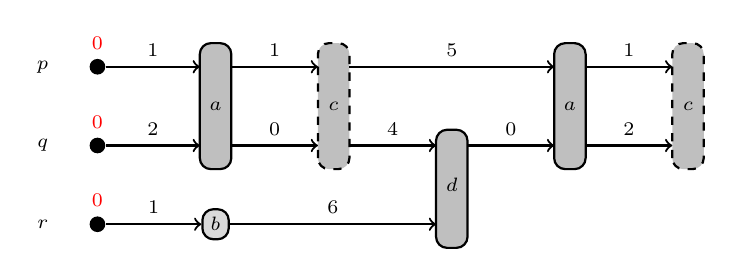
\begin{tikzpicture}[event/.style={rectangle, rounded corners, fill=gray!30, draw, thick, inner sep=3pt}]  
		\node [circle, fill, inner sep=2pt] (10) at (0,0.5) {};
    	\node [circle, fill, inner sep=2pt] (20) at (0,-0.5) {};
		\node [circle, fill, inner sep=2pt] (30) at (0,-1.5) {};

		\node [left] at (-0.5, 0.5) {\scriptsize $p$};
		\node [left] at (-0.5, -0.5) {\scriptsize $q$};
		\node [left] at (-0.5, -1.5) {\scriptsize $r$};

		\node at (0, 0.8) {\scriptsize \textcolor{red}{$0$}};
		\node at (0, -0.2) {\scriptsize \textcolor{red}{$0$}};
		\node at (0, -1.2) {\scriptsize \textcolor{red}{$0$}};

		\draw [rounded corners, fill=gray!50, thick] (1.3, -0.8) rectangle (1.7, 0.8);
    \node at (1.5,0) {\scriptsize $a$};
	\draw [rounded corners, fill=gray!50, thick,dashed] (2.8, -0.8) rectangle (3.2, 0.8);
    \node at (3,0) {\scriptsize $c$};

	\draw [rounded corners, fill=gray!50, thick] (4.3, -1.8) rectangle (4.7, -0.3);
    \node at (4.5,-1) {\scriptsize $d$};

	\draw [rounded corners, fill=gray!50, thick] (5.8, -0.8) rectangle (6.2, 0.8);
    \node at (6,0) {\scriptsize $a$};
	\draw [rounded corners, fill=gray!50, thick,dashed] (7.3, -0.8) rectangle (7.7, 0.8);
    \node at (7.5,0) {\scriptsize $c$};

	\begin{scope}[every node/.style={event}]
		\node (31) at (1.5, -1.5) {\scriptsize $b$};
	
	\end{scope}
	\begin{scope}[->, thick, auto]
		\draw (10) to node {\scriptsize $1$} (1.3,0.5);
		\draw (20) to node {\scriptsize $2$} (1.3,-0.5);
		\draw (30) to node {\scriptsize $1$} (31);
		\draw (1.7, 0.5) to node {\scriptsize $1$} (2.8, 0.5);
		\draw (1.7, -0.5) to node {\scriptsize $0$} (2.8, -0.5);
		\draw (3.2, -0.5) to node {\scriptsize $4$} (4.3, -0.5);
		\draw (31) to node {\scriptsize $6$} (4.3, -1.5);
		\draw (3.2, 0.5) to node {\scriptsize $5$} (5.8, 0.5);
		\draw (4.7, -0.5) to node {\scriptsize $0$} (5.8, -0.5);
		\draw (6.2, 0.5) to node {\scriptsize $1$} (7.3, 0.5);
		\draw (6.2,-0.5) to node {\scriptsize $2$} (7.3, -0.5);
	
	\end{scope}
	
	\end{tikzpicture}
	\caption{Trace representation of a run from Figure~\ref{fig:three-in-one}(a). Each agent has its own timeline (horizontal line), events are shown as boxes, and edge labels indicate time delays.}
\label{fig:trace}
\end{figure}

\paragraph*{Interpreting the Trace Diagram}

Figure~\ref{fig:trace} shows the trace of a run from Example~\ref{eg:three-in-one}. Let's understand each component:

\begin{itemize}
\item \textbf{Agent timelines}: Each horizontal line represents one agent's local timeline. Process $p$ has a timeline at the top, $q$ in the middle, $r$ at the bottom.

\item \textbf{Initial events}: The small filled circles (dots) on the left represent initial events, denoted $\bot_p, \bot_q, \bot_r$. The red numbers above them show initial local times (all 0 in this case).

\item \textbf{Events}: Boxes represent negotiation outcomes. Light gray boxes (like $a$, $b$, $d$) are non-synchronizing events. Darker boxes with dashed borders (like $c$) are time-synchronizing events.

\item \textbf{Time delays}: The numbers on edges show how much local time elapses for that agent between consecutive events. For example:
  \begin{itemize}
  \item $p$ waits 1 unit before participating in $a$
  \item $q$ waits 2 units before participating in $a$
  \item After $a$, $p$ waits 1 more unit before $c$, while $q$ waits 0 units
  \end{itemize}

\item \textbf{Computing timestamps}: We can calculate the local time at any event by summing delays along the path from the initial event. For instance:
  \begin{itemize}
  \item $\tau_p(a) = 0 + 1 = 1$ (initial time plus delay to $a$)
  \item $\tau_q(a) = 0 + 2 = 2$
  \item $\tau_p(c) = 0 + 1 + 1 = 2$
  \item $\tau_q(c) = 0 + 2 + 0 = 2$ (same as $p$ since $c$ is time-synchronizing)
  \end{itemize}
\end{itemize}

\paragraph*{Key Properties of Traces}

The trace representation makes several important aspects explicit:

\begin{enumerate}
\item \textbf{Independence}: Each agent's timeline is separate, showing that agents advance time independently except at time-synchronizing events.

\item \textbf{Synchronization points}: Time-synchronizing events (dashed boxes) span multiple agent timelines, visually showing where times must match.

\item \textbf{Causality}: The left-to-right ordering along each agent's timeline respects causality---events to the right happen after events to the left for that agent.

\item \textbf{Partial ordering}: Events on different agent timelines are only ordered if there's a synchronization relationship. For example, $b$ (for $r$) and the first $a$ (for $p,q$) are concurrent---neither causally depends on the other.
\end{enumerate}

\paragraph*{Formal Definition}

Fix an LTN $\Nn$ and a run:
\[
\rho:= (C_1, v_1) \xra{\Delta_1, e_1} (C_2, v_2) \xra{\Delta_2, e_2} \cdots (C_k, v_k)
\]
starting from configuration $(C_1, v_1)$.

The trace $\tr(\rho)$ is a directed graph $(E_\rho, \{\xra{}_p\}_{p\in P})$ with an initial timestamp assignment $\{\tau^0_p\}_{p\in P}$, where:

\begin{itemize}
\item \textbf{Vertex set} $E_\rho$ contains:
  \begin{itemize}
  \item The negotiation events $\{e_1, e_2, \dots, e_{k-1}\}$ from the run
  \item Special initial events $\{\bot_p\}_{p\in P}$, one per agent
  \end{itemize}

\item \textbf{Edge set} partitioned as $\{\xra{}_p\}_{p \in P}$: There is an edge $e_i \xra{~\theta~}_p e_j$ labeled $\theta$ if:
  \begin{itemize}
  \item $e_j$ is the next event $p$ participates in after $e_i$
  \item Formally: $i < j$, $p \in \dom(e_i) \cap \dom(e_j)$, and no $i < i' < j$ has $p \in \dom(e_{i'})$
  \item The label $\theta = \Delta_i(p) + \Delta_{i+1}(p) + \cdots + \Delta_{j-1}(p)$ is the total time $p$ elapses between $e_i$ and $e_j$
  \end{itemize}

\item \textbf{Initial timestamps} $\tau^0_p = v_1(t_p)$ for each agent $p$
\end{itemize}

Given the trace and its initial timestamps, we can compute the local time at any event $e$ for any agent $p \in \dom(e)$ by summing along the path:
\[
\tau_p(e) = \tau^0_p + \sum_{\text{edges on path from } \bot_p \text{ to } e} \theta
\]

For time-synchronizing events $s$, all participating agents have the same timestamp, so we write $\tau(s)$ for this common value.

\paragraph*{Bidirectional Conversion}

Intuitively, a trace is a labelled partial-order view of a run, similar in spirit to Mazurkiewicz traces or message sequence charts:
vertices are event occurrences, and edges record \emph{the next event seen by each agent} together with the \emph{total time spent in between}.
Thus, forgetting the numeric labels yields the causal skeleton of the run, while keeping them allows us to reconstruct the exact local timestamps.
Time-synchronizing events are special because they force the participating agents' timestamps to coincide, turning the trace into a system of timing constraints.

\paragraph{Run to trace.}
Fix an LTN $\Nn$ with set of agents $P$. Let
\[
\rho \;:=\; (C_0,v_0)\xra{(\Delta_1,e_1)}(C_1,v_1)\xra{(\Delta_2,e_2)}\cdots
\xra{(\Delta_k,e_k)}(C_k,v_k)
\]
be a (finite) run of $\Nn$, where each $e_i$ is an executed outcome (an event) and each $\Delta_i:P\to \mathbb{R}_{\ge 0}$ is the local-delay vector of the $i$-th step.

We define the trace $\tr(\rho)$ as a structure
\[
\tr(\rho) \;=\; (E_\rho,\;(\xra{}_p)_{p\in P},\;(\tau_p^0)_{p\in P})
\]
where:

\begin{enumerate}
\item \textbf{Events.} The event set is
\[
E_\rho \;:=\; \{\bot_p : p\in P\} \;\cup\; \{e_1,\ldots,e_k\}.
\]
The elements $\bot_p$ are fresh symbols (not occurring among the $e_i$) and represent the initial ``dummy event'' of agent $p$.

\item \textbf{Initial timestamps.} For each agent $p\in P$ we set
\[
\tau_p^0 \;:=\; v_0(t_p).
\]

\item \textbf{Per-agent successor edges.} Fix an agent $p\in P$ and consider the indices at which $p$ participates:
\[
I_p \;:=\; \{\, i\in\{1,\ldots,k\} : p\in \dom(e_i)\,\}.
\]
If $I_p=\emptyset$, then $\bot_p$ has no outgoing $\xra{}_p$-edge.

Otherwise write $I_p=\{i_1< i_2<\cdots<i_m\}$. We put:
\begin{itemize}
\item an edge $\bot_p \xra{\theta_{p,0}}_p e_{i_1}$, where
\[
\theta_{p,0} \;:=\; \sum_{j=1}^{i_1} \Delta_j(p),
\]
i.e.\ the total time elapsed locally for $p$ before its first participating event;
\item for every $r\in\{1,\ldots,m-1\}$ an edge
\[
e_{i_r} \xra{\theta_{p,r}}_p e_{i_{r+1}},
\qquad\text{where}\qquad
\theta_{p,r} \;:=\; \sum_{j=i_r+1}^{i_{r+1}} \Delta_j(p).
\]
\end{itemize}
We write $u\xra{\theta}_p u'$ when $(u,u')$ is an edge in the $p$-component with label $\theta$.

\end{enumerate}

\noindent
\textbf{Induced timestamps.} Given $\tr(\rho)$, for any event $e\in E_\rho$ and any agent $p\in P$ such that $e$ lies on the $p$-chain (i.e.\ $e\in\{e_i : i\in I_p\}$), define $\tau_p(e)$ by
\[
\tau_p(e)\;:=\;\tau_p^0 \;+\; \sum \text{(labels along the unique $\xra{}_p$-path from $\bot_p$ to $e$)}.
\]
Equivalently, if $e=e_{i_r}$ then $\tau_p(e)=v_0(t_p)+\sum_{j=1}^{i_r}\Delta_j(p)$.
In particular, for any time-synchronizing event $s$ and any $p,q\in \dom(s)$ we have $\tau_p(s)=\tau_q(s)$ (because $\rho$ satisfies the time-synchronization constraint at $s$).

\medskip

\paragraph{Trace to run.}
Let $\tr=(E,(\xra{}_p)_{p\in P},(\tau_p^0)_{p\in P})$ be a trace.
We say that an initial configuration $(C_0,v_0)$ \emph{matches} the initial timestamps of $\tr$ if
\[
v_0(t_p)=\tau_p^0 \quad\text{for all } p\in P.
\]

Assume $(C_0,v_0)$ matches $\tr$. We now define a canonical run
\[
\rho[(C_0,v_0),\tr]
\]
obtained by choosing any linearization of the trace and executing the corresponding timed steps.

\begin{enumerate}
\item \textbf{The trace order and linearizations.}
For each agent $p$, the relation $\xra{}_p$ is a (finite) directed path starting at $\bot_p$ and visiting exactly the events in which $p$ participates, in the order they appear for $p$.
Let $\prec$ be the strict partial order on $E\setminus\{\bot_p:p\in P\}$ generated by these edges:
\[
e \prec e' \quad\text{if}\quad \exists p\in P \text{ with } e(\xra{}_p)^+ e'.
\]
A \emph{linearization} of $\tr$ is any sequence $(e_1,\ldots,e_k)$ listing all non-initial events exactly once such that $e\prec e'$ implies $e$ appears before $e'$ in the sequence.

\item \textbf{Delays induced by a linearization.}
Fix a linearization $(e_1,\ldots,e_k)$. For each position $i\in\{1,\ldots,k\}$ and each agent $p\in P$, define the local delay
\[
\Delta_i(p)\;:=\;
\begin{cases}
\theta & \text{if } pred_p(e_i)\xra{\theta}_p e_i \text{ is the incoming $p$-edge into } e_i,\\[2pt]
0 & \text{if } p\notin \dom(e_i),
\end{cases}
\]
where $pred_p(e_i)$ denotes the unique predecessor of $e_i$ on the $p$-chain (it is either $\bot_p$ or a previous event of $p$).  
Thus, $\Delta_i$ is a function $P\to \mathbb{R}_{\ge 0}$.

\item \textbf{Executing the steps.}
Starting from $(C_0,v_0)$, execute the events in the chosen order. Concretely, for $i=1,\ldots,k$ let
\[
(C_{i-1},v_{i-1}) \xra{(\Delta_i,e_i)} (C_i,v_i)
\]
be the unique successor configuration obtained by:
\begin{enumerate}
\item letting each agent $p$ elapse $\Delta_i(p)$ time units in its local time (and updating all clocks of $p$ accordingly under the LTN semantics), while agents not in $\dom(e_i)$ elapse $0$;
\item firing the outcome/event $e_i$ from marking $C_{i-1}$ (which updates the marking component to $C_i$ in the standard way);
\item applying the guards/resets of $e_i$ to update the valuation from the post-delay valuation to $v_i$ (again as per the LTN operational semantics).
\end{enumerate}
The resulting sequence is $\rho[(C_0,v_0),\tr]$.

\end{enumerate}

\paragraph{Well-definedness and validity.}
For a fixed linearization, the above construction is \emph{well-defined} because each event $e_i$ has exactly one incoming $\xra{}_p$-edge for each $p\in \dom(e_i)$, hence $\Delta_i$ is uniquely determined.

Whether $\rho[(C_0,v_0),\tr]$ is a \emph{valid run} of $\Nn$ depends on feasibility:
it is a valid run iff every step is enabled when executed, i.e.\ the marking enables $e_i$ and the valuation after applying $\Delta_i$ satisfies the guard of $e_i$ (and time-synchronization constraints, if $e_i$ is time-synchronizing). When this holds for one (equivalently, for every) linearization consistent with $\prec$, we say that $\tr$ is \emph{realizable from $(C_0,v_0)$}.

\paragraph*{A useful viewpoint.}
Once a trace $\tr$ is fixed, the only freedom left in reconstructing a run is the choice of a linearization (a topological order compatible with all $\xra{}_p$ edges). Importantly, \emph{timestamps of events do not depend on the chosen linearization}: $\tau_p(e)$ is determined purely by the unique $\xra{}_p$-path from $\bot_p$ to $e$. This makes traces an ideal object for reasoning about drift, because drift compares timestamps, not interleavings.

The sequence $\rho[(C_0,v_0), \tr]$ is a valid run if and only if all guards are satisfied and synchronization constraints are met.

This trace representation will be the foundation for our tightening algorithm in Section~\ref{sec:tighten}.

\subsection{Tightening a Run}
\label{sec:tighten}

The key idea is that delays larger than $M+1$ contain ''slack'' that can often be reduced. We'll formalize this through a sequence of increasingly complex examples, then define the general tightening procedure.

\subsubsection{Intuition Through Examples}

\paragraph*{Single Agent: Simple Slack Removal}

Figure~\ref{fig:trace-1} shows the simplest case---a single agent with some large delays.

\begin{figure}[t]
\centering
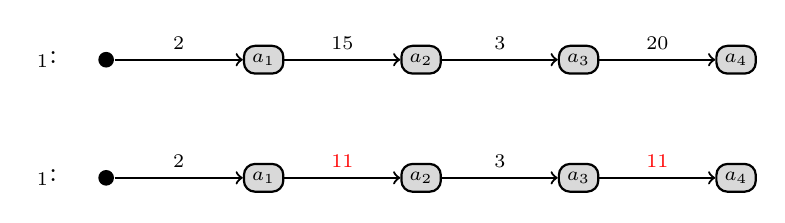
\begin{tikzpicture}[event/.style={rectangle, rounded corners, fill=gray!30, draw, thick, inner sep=3pt}]
    
    \node [circle, fill, inner sep=2pt] (0) at (0,0) {};
    \begin{scope}[every node/.style={event}]
        
        \node (1) at (2,0) {\scriptsize $a_1$};
        \node (2) at (4,0) {\scriptsize $a_2$};
        \node (3) at (6,0) {\scriptsize $a_3$};
        \node (4) at (8,0) {\scriptsize $a_4$};
    \end{scope}

    \begin{scope}[->, thick, auto ]
        \draw (0) to node {\scriptsize $2$} (1);
        \draw (1) to node {\scriptsize $15$} (2);
        \draw (2) to node {\scriptsize $3$} (3);
        \draw (3) to node {\scriptsize $20$} (4);
    \end{scope} 


    \node [left] at (-0.5, 0) { $\tr_1$:};
    \begin{scope}[yshift=-1.5cm]
        \node [circle, fill, inner sep=2pt] (0) at (0,0) {};
        \begin{scope}[every node/.style={event}]
            \node (1) at (2,0) {\scriptsize $a_1$};
            \node (2) at (4,0) {\scriptsize $a_2$};
            \node (3) at (6,0) {\scriptsize $a_3$};
            \node (4) at (8,0) {\scriptsize $a_4$};
        \end{scope}
    
        \begin{scope}[->, thick, auto ]
            \draw (0) to node {\scriptsize $2$} (1);
            \draw (1) to node {\scriptsize \textcolor{red}{$11$}} (2);
            \draw (2) to node {\scriptsize $3$} (3);
            \draw (3) to node {\scriptsize \textcolor{red}{$11$}} (4);
        \end{scope} 
    

        \node [left] at (-0.5, 0) { $\overline{\tr}_1$:};
    \end{scope}
\end{tikzpicture}
\caption{Tightening a single-agent trace with $M = 10$. Delays larger than $M+1 = 11$ are reduced to exactly $11$.}
\label{fig:trace-1}
\end{figure}

With maximum constant $M = 10$, any delay larger than $M+1 = 11$ contains slack. Here's why we can reduce it:

\begin{itemize}
\item \textbf{Clock values}: All guards compare clocks against constants $\leq M = 10$. 

\item \textbf{Clock regions}: For verification purposes, we only need to distinguish:
  \begin{enumerate}
  \item Clock values in $\{0, 1, 2, \ldots, M\}$ (individually)
  \item Clock values $ > M$ (all equivalent from the guard's perspective)
  \end{enumerate}

\item \textbf{Key insight}: After time $M+1$, any clock that hasn't been reset will have value $> M$. Whether its value is $15$, $20$, or $100$ doesn't matter---it will satisfy the same set of guards (those with $x > c$ for $c \leq M$, and fail those with $x \leq c$ or $x = c$).

\item \textbf{Reduction}: In trace $\tr_1$:
  \begin{itemize}
  \item The delay from $a_1$ to $a_2$ is $15 = 11 + 4$. We can reduce it to $11$.
  \item The delay from $a_3$ to $a_4$ is $20 = 11 + 9$. We can reduce it to $11$.
  \item The delay from $\bot$ to $a_1$ is $2 \leq 11$, so we keep it.
  \item The delay from $a_2$ to $a_3$ is $3 \leq 11$, so we keep it.
  \end{itemize}

\item \textbf{Preservation}: The tightened trace $\overline{\tr}_1$ has the same enabling of outcomes as $\tr_1$, because at each event:
  \begin{itemize}
  \item Clocks with value $\leq M$ have the same exact value
  \item Clocks with value $> M$ still have value $> M$ (just a smaller value $> M$)
  \end{itemize}
\end{itemize}

This gives us the tightened trace $\overline{\tr}_1$ shown at the bottom of Figure~\ref{fig:trace-1}.

\paragraph*{Multiple Agents: Synchronization Constraints}

Now consider two agents with a time-synchronizing event. Figure~\ref{fig:trace-2} shows why this is more subtle.

\begin{figure}[h]
\centering
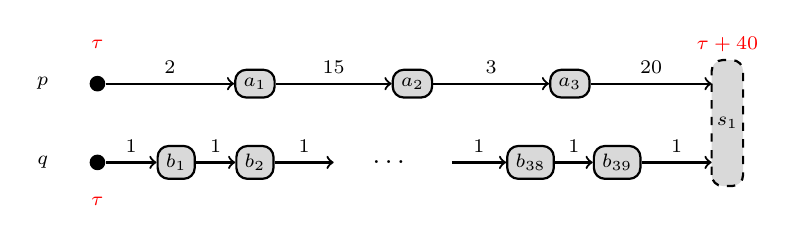
\begin{tikzpicture}[event/.style={rectangle, rounded corners, fill=gray!30, draw, thick, inner sep=3pt}]  
    \node [circle, fill, inner sep=2pt] (i0) at (0,0.5) {};
    \node [circle, fill, inner sep=2pt] (i1) at (0,-0.5) {};

    \draw [rounded corners, fill=gray!30, thick, dashed]   (7.8, -0.8) rectangle (8.2, 0.8);
    \node at (8, 0) {\scriptsize $s_1$};

    \node [left] at (-0.5, 0.5) {\scriptsize $p$};
    \node [left] at (-0.5, -0.5) {\scriptsize $q$};
    \begin{scope}[every node/.style={event}]
        \node (11) at (2,0.5) {\scriptsize $a_1$};
        \node (12) at (4,0.5) {\scriptsize $a_2$};
        \node (13) at (6,0.5) {\scriptsize $a_3$};

        \node (21) at (1, -0.5) {\scriptsize $b_1$};
        \node (22) at (2, -0.5) {\scriptsize $b_2$};
        \node (2a) at (5.5, -0.5) {\scriptsize $b_{38}$};
        \node (2b) at (6.6, -0.5 ) {\scriptsize $b_{39}$};
        
    \end{scope}

    \begin{scope}[->, thick, auto]
        \draw (i0) to node {\scriptsize $2$} (11);
        \draw (11) to node {\scriptsize $15$} (12);
        \draw (12) to node {\scriptsize $3$} (13);
        \draw (13) to node {\scriptsize $20$} (7.8, 0.5);
        \draw (i1) to node{\scriptsize $1$} (21);
        \draw (21) to node {\scriptsize $1$} (22);
        \draw (22) to node {\scriptsize $1$} (3,-0.5);
        \draw (4.5,-0.5) to node {\scriptsize $1$} (2a);
        \draw (2a) to node {\scriptsize $1$} (2b);
        \draw (2b) to node {\scriptsize $1$} (7.8, -0.5);
    
    \end{scope}

    \node at (3.7, -0.5) {$\dots$};
    \node [red] at (0, 1) {\scriptsize $\tau$};
    \node [red] at (0,-1) {\scriptsize $\tau$};
    \node [red] at (8, 1) {\scriptsize $\tau+40$};
\end{tikzpicture}
\caption{Two-agent trace with $M = 10$. The synchronization at $s_1$ prevents tightening, even though $p$ has large delays.}
\label{fig:trace-2}
\end{figure}

Both agents start at local time $\tau$. Process $p$ has slack (delays of $15$ and $20$, both $> 11$), but we \emph{cannot} reduce them! Here's why:

\begin{itemize}
\item Agent $p$ reaches $s_1$ at time $\tau + 40 = \tau + 2 + 15 + 3 + 20$
\item Agent $q$ reaches $s_1$ at time $\tau + 40 = \tau + 1 + 1 + \cdots + 1$ (40 events, each 1 unit apart, but only a few shown)
\item Since $s_1$ is time-synchronizing, we must have $\tau_p(s_1) = \tau_q(s_1)$

\item If we reduce $p$'s delays (say, to $11$ each), $p$ reaches $s_1$ at time $\tau + 2 + 11 + 3 + 11 = \tau + 27$
\item But $q$ still reaches $s_1$ at time $\tau + 40$
\item Now $\tau_p(s_1) \neq \tau_q(s_1)$, violating the synchronization constraint!
\end{itemize}

The lesson: we can only reduce delays by an amount that \emph{all} agents participating in future synchronizations can accommodate.

This trace $\tr_2$ is already tight---there's no slack we can safely remove.

\paragraph*{Multiple Agents with Different Slacks}

Figure~\ref{fig:trace-3} shows a more interesting case where both agents have slack, but different amounts.

\begin{figure}
\centering
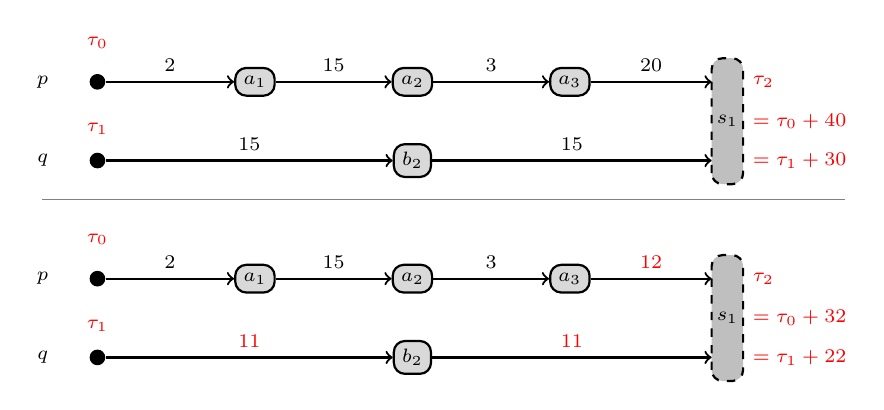
\begin{tikzpicture}[event/.style={rectangle, rounded corners, fill=gray!30, draw, thick, inner sep=3pt}]  
    \node [circle, fill, inner sep=2pt] (10) at (0,0.5) {};
    \node [circle, fill, inner sep=2pt] (21) at (0,-0.5) {};

    \begin{scope}[every node/.style={event}]
        \node (11) at (2,0.5) {\scriptsize $a_1$};
        \node (12) at (4,0.5) {\scriptsize $a_2$};
        \node (13) at (6,0.5) {\scriptsize $a_3$};
        \node (22) at (4,-0.5) {\scriptsize $b_2$};
    \end{scope}
    \draw [rounded corners, fill=gray!50, thick, dashed] (7.8, -0.8) rectangle (8.2, 0.8);
    \node at (8,0) {\scriptsize $s_1$};

    \begin{scope}[->,thick,auto]
        \draw (10) to node {\scriptsize $2$} (11);
        \draw (11) to node {\scriptsize $15$} (12);
        \draw (12) to node {\scriptsize $3$} (13);
        \draw (13) to node {\scriptsize $20$} (7.8, 0.5);
        \draw (21) to node {\scriptsize $15$} (22);
        \draw (22) to node {\scriptsize $15$} (7.8, -0.5);
    \end{scope}

    \node [red] at (0, 1) {\scriptsize $\tau_0$};
    \node [red] at (0, -0.1) {\scriptsize $\tau_1$};
    \node [red, right] at (8.2, 0.5) {\scriptsize $\tau_2$};
    \node [red, right] at (8.2, 0) {\scriptsize $= \tau_0 + 40$};
    \node [red, right] at (8.2, -0.5) {\scriptsize $= \tau_1 + 30$};
    
    \node [left] at (-0.5,0.5) {\scriptsize $p$};
    \node [left] at (-0.5,-0.5) {\scriptsize $q$};

    \draw [thin, gray] (-0.7, -1) -- (9.5, -1);
   
    \begin{scope}[yshift=-2.5cm]
        \node [circle, fill, inner sep=2pt] (10) at (0,0.5) {};
    \node [circle, fill, inner sep=2pt] (21) at (0,-0.5) {};

    \begin{scope}[every node/.style={event}]
        \node (11) at (2,0.5) {\scriptsize $a_1$};
        \node (12) at (4,0.5) {\scriptsize $a_2$};
        \node (13) at (6,0.5) {\scriptsize $a_3$};
        \node (22) at (4,-0.5) {\scriptsize $b_2$};
    \end{scope}
    \draw [rounded corners, fill=gray!50, thick, dashed] (7.8, -0.8) rectangle (8.2, 0.8);
    \node at (8,0) {\scriptsize $s_1$};

    \begin{scope}[->,thick,auto]
        \draw (10) to node {\scriptsize $2$} (11);
        \draw (11) to node {\scriptsize $15$} (12);
        \draw (12) to node {\scriptsize $3$} (13);
        \draw  (13) to node {\scriptsize \textcolor{red}{$12$}} (7.8, 0.5);
        \draw  (21) to node {\scriptsize \textcolor{red}{$11$}} (22);
        \draw  (22) to node {\scriptsize \textcolor{red}{$11$}} (7.8, -0.5);
    \end{scope}

    \node [red] at (0, 1) {\scriptsize $\tau_0$};
    \node [red] at (0, -0.1) {\scriptsize $\tau_1$};
    \node [red, right] at (8.2, 0.5) {\scriptsize $\tau_2$};
    \node [red, right] at (8.2, 0) {\scriptsize $= \tau_0 + 32$};
    \node [red, right] at (8.2, -0.5) {\scriptsize $= \tau_1 + 22$};
    
    \node [left] at (-0.5,0.5) {\scriptsize $p$};
    \node [left] at (-0.5,-0.5) {\scriptsize $q$};

    
    \end{scope}

\end{tikzpicture}
\caption{Above: Trace $\tr_3$ with $M = 10$. Agent $q$ has less slack than $p$. Below: Tightened trace $\overline{\tr}_3$ reduces both by the minimum slack (8 units).}
\label{fig:trace-3}
\end{figure}

Let's compute the slack for each agent independently:

\begin{itemize}
\item \textbf{Agent $p$'s slack}:
  \begin{itemize}
  \item Edge $a_1 \to a_2$: delay 15, slack = $15 - 11 = 4$
  \item Edge $a_3 \to s_1$: delay 20, slack = $20 - 11 = 9$
  \item Total slack: $4 + 9 = 13$
  \end{itemize}

\item \textbf{Agent $q$'s slack}:
  \begin{itemize}
  \item Edge $\bot_q \to b_2$: delay 15, slack = $15 - 11 = 4$
  \item Edge $b_2 \to s_1$: delay 15, slack = $15 - 11 = 4$
  \item Total slack: $4 + 4 = 8$
  \end{itemize}
\end{itemize}

Now here's the crucial point: if we reduce by more than 8 units, $q$ won't be able to reach the synchronization time. So we reduce by exactly 8:

\begin{itemize}
\item In the original trace:
  \begin{itemize}
  \item $\tau_p(s_1) = \tau_0 + 40$
  \item $\tau_q(s_1) = \tau_1 + 30$
  \item Synchronization requires: $\tau_0 + 40 = \tau_1 + 30$, so $\tau_1 = \tau_0 + 10$
  \end{itemize}

\item After reducing by 8:
  \begin{itemize}
  \item $\tau_p(s_1) = \tau_0 + 32$ (reduced from 40)
  \item $\tau_q(s_1) = \tau_1 + 22$ (reduced from 30)
  \item Still synchronized: $\tau_0 + 32 = \tau_1 + 22$ when $\tau_1 = \tau_0 + 10$ $\checkmark$
  \end{itemize}
\end{itemize}

The tightened trace $\overline{\tr}_3$ shown in the bottom of Figure~\ref{fig:trace-3} achieves this by:
\begin{itemize}
\item Reducing $p$'s delay from $a_3$ to $s_1$ from 20 to 12 (saves 8)
\item Reducing $q$'s delays from 15 to 11 each (saves 4 + 4 = 8)
\end{itemize}

\paragraph*{Future Synchronizations Constrain Present Slacks}

Our final example (Figure~\ref{fig:trace-4}) reveals perhaps the most subtle aspect of tightening: slack can be limited by \emph{future} synchronizations, not just past ones.

\begin{figure}
\centering
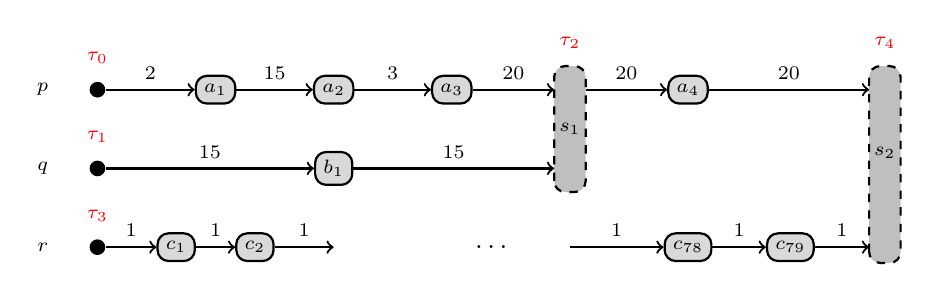
\begin{tikzpicture}[event/.style={rectangle, rounded corners, fill=gray!30, draw, thick, inner sep=3pt}]  
    \node [circle, fill, inner sep=2pt] (10) at (0,0.5) {};
    \node [circle, fill, inner sep=2pt] (20) at (0,-0.5) {};
    \node [circle, fill, inner sep=2pt] (30) at (0,-1.5) {};

    \node [left] at (-0.5, 0.5) {\scriptsize $p$};
    \node [left] at (-0.5, -0.5) {\scriptsize $q$};
    \node [left] at (-0.5, -1.5) {\scriptsize $r$};

    \begin{scope}[every node/.style={event}]
        \node (11) at (1.5,0.5) {\scriptsize $a_1$};
        \node (12) at (3,0.5) {\scriptsize $a_2$};
        \node (13) at (4.5,0.5) {\scriptsize $a_3$};
        \node (14) at (7.5, 0.5) {\scriptsize $a_4$};
        \node (21) at (3,-0.5) {\scriptsize $b_1$};
        \node (31) at (1,-1.5) {\scriptsize $c_1$};
        \node (32) at (2,-1.5) {\scriptsize $c_2$};
        \node (3a) at (7.5, -1.5) {\scriptsize $c_{78}$};
        \node (3b) at (8.8, -1.5) {\scriptsize $c_{79}$};    
    \end{scope}
    \draw [rounded corners, fill=gray!50, thick, dashed] (5.8, -0.8) rectangle (6.2, 0.8);
    \node at (6,0) {\scriptsize $s_1$};
    \draw [rounded corners, fill=gray!50, thick, dashed] (9.8, -1.7) rectangle (10.2, 0.8);
    \node at (10,-0.3) {\scriptsize $s_2$};    
    
    \begin{scope}[->,thick, auto]
        \draw (10) to node {\scriptsize $2$} (11);
        \draw (11) to node {\scriptsize $15$} (12);
        \draw (12) to node {\scriptsize $3$} (13);
        \draw (13) to node {\scriptsize $20$} (5.8, 0.5);
        \draw (6.2, 0.5) to node {\scriptsize $20$} (14);
        \draw (14) to node {\scriptsize $20$} (9.8, 0.5);
        \draw (20) to node {\scriptsize $15$} (21);
        \draw (21) to node {\scriptsize $15$} (5.8, -0.5);
        \draw (30) to node {\scriptsize $1$} (31);
        \draw (31) to node {\scriptsize $1$} (32);
        \draw (32) to node {\scriptsize $1$} (3, -1.5);
        \draw (6, -1.5) to node {\scriptsize $1$} (3a);
        \draw (3a) to node {\scriptsize $1$} (3b);
        \draw (3b) to node {\scriptsize $1$} (9.8, -1.5);
    \end{scope}
    \node at (5, -1.5) {$\dots$};
    
    \node [red] at (0,0.9) {\scriptsize $\tau_0$};
    \node [red] at (0, -0.1) {\scriptsize $\tau_1$};
    \node [red] at (6, 1.1) {\scriptsize $\tau_2$};
    \node [red] at (0, -1.1) {\scriptsize $\tau_3$};
    \node [red] at (10, 1.1) {\scriptsize $\tau_4$};
    
 
\end{tikzpicture}
\caption{Trace $\tr_4$ with $M = 10$. Despite slack in $p$ and $q$ before $s_1$, the trace is tight because $r$ has no slack before $s_2$.}
\label{fig:trace-4}
\end{figure}

This trace extends $\tr_3$ with a second synchronization $s_2$ between $p$ and $r$. Let's analyze it:

\begin{itemize}
\item \textbf{Before $s_1$}: Just like in $\tr_3$:
  \begin{itemize}
  \item $p$ has slack 13 (from delays 15 and 20)
  \item $q$ has slack 8 (from two delays of 15)
  \end{itemize}

\item \textbf{Between $s_1$ and $s_2$}:
  \begin{itemize}
  \item $p$ has large delays (20 twice), slack = $(20-11) + (20-11) = 18$
  \item $r$ has only small delays (many 1's), no slack at all!
  \end{itemize}

\item \textbf{The critical constraint}: At $s_2$, we need $\tau_p(s_2) = \tau_r(s_2)$. 
  \begin{itemize}
  \item If we reduce any of $p$'s delays, $\tau_p(s_2)$ decreases
  \item But $r$ has no slack---we cannot reduce $\tau_r(s_2)$
  \item Therefore, we cannot reduce $p$'s delays at all!
  \end{itemize}

\item \textbf{Backward propagation}: This constraint propagates backward through $s_1$:
  \begin{itemize}
  \item We can't reduce $p$'s delays to $s_2$
  \item At $s_1$, $p$ and $q$ must synchronize
  \item So we also can't reduce $q$'s delays to $s_1$ (otherwise $s_1$ wouldn't synchronize)
  \end{itemize}
\end{itemize}

Even though $p$ and $q$ have apparent slack before $s_1$, the trace $\tr_4$ is already tight! The future synchronization $s_2$ constrains what we can do now.

\subsubsection{The Slack Graph}

The examples above motivate our formal definition of slack. The key idea is to build a graph that captures both:
\begin{enumerate}
\item How much each edge can be reduced (\emph{forward} information about available slack)
\item How future synchronizations constrain present reductions (\emph{backward} information via synchronization points)
\end{enumerate}

\paragraph*{What ``slack'' measures.}
For each agent, every local edge $e \xra{\theta}_p e'$ can be written as
\[
\theta = \underbrace{\min(\theta, M{+}1)}_{\text{``relevant'' part}} \;+\;
\underbrace{\max(0,\theta-(M{+}1))}_{\text{slack}},
\]
where the relevant part is the only part that guards can ever observe.
Tightening is the process of removing slack wherever possible, while still respecting future time-synchronizations.

\begin{definition}[Slack Graph]
Given a trace $\tr$ with maximum constant $M$, its \emph{slack graph} $\Sl(\tr)$ is constructed as follows:

\begin{enumerate}
\item \textbf{Start with the trace}: Begin with all vertices and edges from $\tr$

\item \textbf{Compute slack on each edge}: For every edge $e \xra{\theta}_p e'$ in $\tr$:
  \[
  \text{slack} = \begin{cases}
    0 & \text{if } \theta \leq M+1 \\
    \theta - (M+1) & \text{if } \theta > M+1
  \end{cases}
  \]
  Replace the label $\theta$ with this slack value.

\item \textbf{Add back edges}: For every agent $p$ and every pair of time-synchronizing events $e_i, e_j$ with $p \in \dom(e_i) \cap \dom(e_j)$:
  \begin{itemize}
  \item If $e_i (\xra{}_p)^+ e_j$ (meaning $e_i$ occurs before $e_j$ in $p$'s timeline)
  \item Add a back edge $e_j \xra{0}_p e_i$ with weight 0
  \end{itemize}
\end{enumerate}
\end{definition}

\paragraph*{What problem is $\Sl(\tr)$ solving? (difference constraints / potentials).}
The slack graph is not a heuristic device: it encodes a system of \emph{difference constraints}
whose solutions correspond exactly to the globally consistent ways of shaving slack.

Fix a trace $\tr$ and write $\tau(e)$ for the timestamp of an event occurrence $e$.
A \emph{tightening} chooses, for each event $e$, a reduction amount $\delta(e)\ge 0$ and sets
\[
\overline{\tau}(e)\ :=\ \tau(e)-\delta(e).
\]
Intuitively, $\delta(e)$ measures how far we shift $e$ to the left.
For time-synchronizing events $s$, the value $\delta(s)$ must be the \emph{same} for all participating agents,
because $\overline{\tau}_p(s)=\overline{\tau}_q(s)$ must still hold after tightening.

Now consider a forward edge $e \xra{\theta}_p e'$ of the trace.
Only the part of $\theta$ above $M{+}1$ is ``removable'': the available slack on this edge is
$\mathrm{slack}(e\xra{\theta}_p e')=\max(0,\theta-(M{+}1))$.
If we reduce the timestamp of $e'$ by $\delta(e')$ and of $e$ by $\delta(e)$, then the local delay on this edge
is reduced by exactly $\delta(e')-\delta(e)$.
Hence feasibility imposes the inequality
\[
\delta(e')-\delta(e)\ \le\ \mathrm{slack}(e\xra{\theta}_p e') .
\]
Rearranging gives a standard difference constraint:
\[
\delta(e')\ \le\ \delta(e)\ +\ \mathrm{slack}(e\xra{\theta}_p e') .
\]
This is precisely what the \emph{weighted forward edges} of $\Sl(\tr)$ encode.

\smallskip
\emph{Back edges} encode the second kind of feasibility constraint: if $s \prec_p s'$ are consecutive
time-synchronizing events on agent $p$, then tightening cannot move the earlier anchor more than the later one
(otherwise some intermediate local delay would become negative).
Formally this gives
\[
\delta(s)\ \le\ \delta(s') ,
\]
which is exactly the constraint encoded by a back edge $s' \xra{0}_p s$ in $\Sl(\tr)$.

\paragraph*{Intended meaning of $\sigma(s)$.}
For a time-synchronizing event $s$, define
\[
\sigma(s)\ :=\ \min_{p\in\dom(s)}\ \mathrm{dist}_{\Sl(\tr)}(\bot_p,s),
\]
i.e.\ the minimum (over sources $\bot_p$) of the shortest-path distance to $s$ in $\Sl(\tr)$.
The intended meaning is:
\begin{quote}
$\sigma(s)$ is the \emph{maximum} amount by which the timestamp of $s$ can be reduced while keeping all
guards and all time-synchronizations satisfiable.
\end{quote}

\paragraph*{Why shortest paths compute the maximum reduction.}
Every directed path $\pi$ from some $\bot_p$ to $s$ in $\Sl(\tr)$ yields (by summing the edge inequalities along $\pi$)
an upper bound of the form $\delta(s)\le w(\pi)$ for \emph{every feasible tightening} $\delta$.
Therefore $\delta(s)$ is bounded by the \emph{minimum} of these upper bounds, i.e.\ by the shortest-path distance.
Conversely, setting $\delta(e)$ to be the shortest-path distance from the set of sources $\{\bot_p\}$ to $e$
satisfies all edge inequalities of $\Sl(\tr)$ (the usual potential property of shortest-path distances),
hence gives a feasible tightening that achieves $\delta(s)=\sigma(s)$.
This is the sense in which $\Sl(\tr)$ is a potentials construction: it computes the componentwise-maximal feasible reduction.

\paragraph*{Why back edges are needed.}
Slack is not only constrained by the past. If an agent $p$ participates in two time-synchronizing events $s \prec s'$, then shifting $s'$ earlier may force $s$ earlier as well, because the intermediate local timeline of $p$ must remain nonnegative. Back edges encode exactly this ``future constraint propagates backwards'' phenomenon, and allow us to compute globally consistent time reductions by a shortest-path style computation.

\paragraph*{Understanding the Construction}

Let's see why each component is necessary:

\begin{itemize}
\item \textbf{Slack values}: An edge with slack 0 means ''this delay cannot be reduced'' (it's already at the minimum safe value $\leq M+1$). An edge with slack 5 means ''we could reduce this delay by up to 5 units while maintaining clock values $> M$ where needed.''

\item \textbf{Back edges}: These propagate constraints from future synchronizations back to earlier events. In trace $\tr_4$, the back edge from $s_2$ to $s_1$ ensures that we recognize: ''if we can't reduce delays to $s_2$, we also can't reduce delays to $s_1$.''
\end{itemize}

\paragraph*{Example: Slack Graph of $\tr_4$}

Let's construct $\Sl(\tr_4)$ step by step:

\begin{enumerate}
\item \textbf{Forward edges with slack}:
  \begin{align*}
    \bot_p \xra{0}_p a_1 \quad &\text{(delay 2, slack 0)} \\
    a_1 \xra{4}_p a_2 \quad &\text{(delay 15, slack 4)} \\
    a_2 \xra{0}_p a_3 \quad &\text{(delay 3, slack 0)} \\
    a_3 \xra{9}_p s_1 \quad &\text{(delay 20, slack 9)} \\
    s_1 \xra{9}_p a_4 \quad &\text{(delay 20, slack 9)} \\
    a_4 \xra{9}_p s_2 \quad &\text{(delay 20, slack 9)} \\
    \bot_q \xra{4}_q b_1 \quad &\text{(delay 15, slack 4)} \\
    b_1 \xra{4}_q s_1 \quad &\text{(delay 15, slack 4)} \\
    \bot_r \xra{0}_r c_1, c_1 \xra{0}_r c_2, \ldots, c_{79} \xra{0}_r s_2 \quad &\text{(all delays 1, all slack 0)}
  \end{align*}

\item \textbf{Back edges}:
  \begin{itemize}
  \item $s_2 \xra{0}_p s_1$ (since $s_1 \xra{}_p^+ s_2$ and both are time-synchronizing for $p$)
  \end{itemize}
\end{enumerate}

This slack graph explicitly shows that there's a zero-weight path from $\bot_r$ through all the $c$ events to $s_2$, and then via the back edge to $s_1$. This is why the trace is tight!

\begin{definition}[Tight Traces]
A trace $\tr$ is \emph{tight} if for every time-synchronizing event $s$, there exists an agent $p \in \dom(s)$ and a path of total weight 0 in $\Sl(\tr)$ from the initial event $\bot_p$ to $s$.
\end{definition}

This definition formalizes our intuition: a trace is tight when we cannot reduce the timestamp of any synchronization point without violating some constraint.

Intuitively, a trace is tight if every time-synchronizing event already has an ``explanation'' path from some start that uses only relevant delays (each $\le M{+}1$), i.e.\ there is no remaining slack that could pull it further to the left.

\paragraph*{Computing Shortest Paths}

For a time-synchronizing event $s$ and agent $p \in \dom(s)$, let $\sigma_p(s)$ denote the weight of the shortest path from $\bot_p$ to $s$ in $\Sl(\tr)$. Define:
\[
\sigma(s) := \min_{p \in \dom(s)} \{\sigma_p(s)\}
\]

%This value $\sigma(s)$ tells us the maximum amount by which we can safely reduce the timestamp of event $s$.
This value $\sigma(s)$ is the (componentwise) maximal feasible reduction of the timestamp of $s$.

Figure~\ref{fig:slack-shortest-paths} shows these shortest paths for our example traces:

\begin{figure}
    \centering
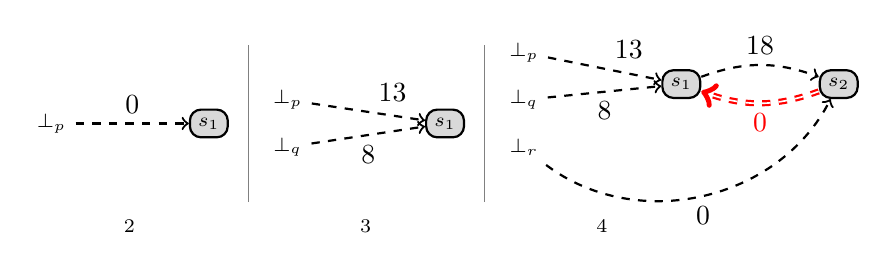
\begin{tikzpicture}[event/.style={rectangle, rounded corners, fill=gray!30, draw, thick, inner sep=3pt}]  

    

    \begin{scope}[xshift=3cm]
        \node (0) at (0,0) {\scriptsize $\bot_p$};
        \begin{scope}[every node/.style={event}]
            \node (1) at (2,0) {\scriptsize $s_1$};
        \end{scope}
        \begin{scope}[->, thick, dashed, auto]
            \draw (0) to node {$0$} (1);
        \end{scope}
        \node at (1, -1.3) {$\tr_2$};
        \draw [thin, gray] (2.5, -1) to (2.5, 1);
    \end{scope}

    \begin{scope}[xshift=6cm]
        \node (0) at (0,0.3) {\scriptsize $\bot_p$};
        \node (1) at (0,-0.3) {\scriptsize $\bot_q$};
        \begin{scope}[every node/.style={event}]
            \node (2) at (2, 0) {\scriptsize $s_1$};
        \end{scope}
        \begin{scope}[->, thick, dashed, auto]
            \draw (0) to node  {$13$} (2);
            \draw (1) to node [below] {$8$} (2);
        \end{scope}
        \node at (1, -1.3) {$\tr_3$};
        \draw [thin, gray] (2.5, -1) to (2.5, 1);
    \end{scope}
    
    \begin{scope}[xshift=9cm]
        \node (0) at (0,0.9) {\scriptsize $\bot_p$};
        \node (1) at (0,0.3) {\scriptsize $\bot_q$};
        \node (3) at (0,-0.3) {\scriptsize $\bot_r$};
        \begin{scope}[every node/.style={event}]
            \node (2) at (2, 0.5) {\scriptsize $s_1$};
            \node (4) at (4, 0.5) {\scriptsize $s_2$};
        \end{scope}

        \begin{scope}[->, thick, dashed, auto]
            \draw (0) to node  {$13$} (2);
            \draw (1) to node [below] {$8$} (2);
            \draw (2) to [bend left=20] node {$18$} (4);
            \draw (3) to [bend right=50] node [below] {$0$} (4);
            \draw [red, double] (4) to [bend left=20] node {$0$} (2); 
        \end{scope}
        \node at (1, -1.3) {$\tr_4$};
    \end{scope}
\end{tikzpicture}
\caption{Shortest weighted paths to synchronizing events in slack graphs. The red double arrow in $\tr_4$ is a back edge that makes both $\sigma(s_1)$ and $\sigma(s_2)$ equal to 0.}
\label{fig:slack-shortest-paths}
\end{figure}

\begin{itemize}
\item \textbf{Trace $\tr_2$}: The path from $\bot_p$ to $s_1$ through the 39 $b$ events (each with delay 1, slack 0) has weight 0. So $\sigma(s_1) = 0$ and the trace is already tight.

\item \textbf{Trace $\tr_3$}: 
  \begin{itemize}
  \item From $\bot_p$: $\bot_p \xra{0} a_1 \xra{4} a_2 \xra{0} a_3 \xra{9} s_1$, total weight 13
  \item From $\bot_q$: $\bot_q \xra{4} b_2 \xra{4} s_1$, total weight 8
  \item So $\sigma(s_1) = \min(13, 8) = 8$
  \end{itemize}
  We can reduce timestamps by 8 units, as shown in Figure~\ref{fig:trace-3}.

\item \textbf{Trace $\tr_4$}:
  \begin{itemize}
  \item The shortest path to $s_2$ from $\bot_r$ has weight 0 (through all the small delays)
  \item The back edge makes the shortest path to $s_1$ also 0
  \item So $\sigma(s_1) = \sigma(s_2) = 0$, and the trace is tight
  \end{itemize}
\end{itemize}

\subsubsection{Properties of the $\sigma$ Function}

Before presenting the tightening algorithm, we need to understand how $\sigma$ values relate across consecutive synchronizations.

\begin{lemma}[Monotonicity of $\sigma$]\label{lem:sigma-monotone}
Let $p \in P$ and let $s, s'$ be time-synchronizing events for $p$ such that $s (\xra{}_p)^+ s'$ (meaning $s$ occurs before $s'$ in $p$'s timeline) and there is no other time-synchronizing event for $p$ between $s$ and $s'$. Then:
\begin{enumerate}
\item $\sigma(s) \leq \sigma(s')$ (non-decreasing along agent timelines)
\item $\sigma(s') \leq \sigma(s) + \theta_p$ where $\theta_p$ is the total slack for $p$ between $s$ and $s'$
\end{enumerate}
\end{lemma}

\begin{proof}
\textbf{Part 1}: By construction of $\Sl(\tr)$, there is a back edge $s' \xra{0}_p s$ with weight 0. Therefore:
\[
\sigma(s) \leq \sigma(s') + 0 = \sigma(s')
\]
Since $\sigma(\cdot)$ is defined as the minimum shortest path distance, and we have a path from any $\bot_q$ to $s'$ that can be extended via the back edge to $s$, we get $\sigma(s) \leq \sigma(s')$.

\textbf{Part 2}: Consider a shortest path from some $\bot_q$ to $s$ witnessing $\sigma(s)$. We can extend this path:
\begin{itemize}
\item From $s$ to $s'$ along $p$'s timeline, accumulating slack $\theta_p$
\item This gives a path from $\bot_q$ to $s'$ of weight $\sigma(s) + \theta_p$
\item By definition of $\sigma(s')$ as the minimum, we have $\sigma(s') \leq \sigma(s) + \theta_p$
\end{itemize}
\qed
\end{proof}

\paragraph*{Why This Matters}

This lemma tells us that we can always ''pay for'' a reduction at a later synchronization $s'$ using slack accumulated between $s$ and $s'$, as long as $\sigma(s) = 0$ (the earlier synchronization is already tight). This is the key to our tightening algorithm.

\subsubsection{The Tightening Algorithm}

We can now state the main result about tightening:

\begin{lemma}[Tightening Lemma]\label{lem:tightening}
From every trace $\tr$, we can construct a trace $\overline{\tr}$ such that:
\begin{enumerate}
\item \textbf{Reduced timestamps}: For every time-synchronizing event $s$:
  \[
  \overline{\tau}(s) = \tau(s) - \sigma(s)
  \]
  where $\tau(s)$ and $\overline{\tau}(s)$ are the timestamps of $s$ in $\tr$ and $\overline{\tr}$ respectively.

\item \textbf{Preserved small delays}: For every edge $e \xra{t}_p e'$ in $\tr$ with $t \leq M+1$:
  \[
  e \xra{t}_p e' \text{ in } \overline{\tr} \text{ as well}
  \]
  (Delays at most $M+1$ are unchanged)

\item \textbf{Preserved validity}: For any configuration $(C,v)$ matching the initial timestamps of $\tr$:
  \[
  \rho[(C,v), \tr] \text{ is a valid run} \quad \Leftrightarrow \quad \rho[(C,v), \overline{\tr}] \text{ is a valid run}
  \]
\end{enumerate}
\end{lemma}

\begin{proof}[Proof sketch]
The algorithm proceeds by distributing the reduction $\sigma(s)$ across the edges leading to each synchronization $s$:

\begin{enumerate}
\item \textbf{Identify reductions}: For each time-synchronizing event $s$, compute $\sigma(s)$ using shortest paths in $\Sl(\tr)$.

\item \textbf{Distribute reductions}: For each agent $p \in \dom(s)$, reduce the delays on edges with non-zero slack along the path from $\bot_p$ (or from the previous synchronization) to $s$, distributing the total reduction of $\sigma(s)$.

\item \textbf{Update timestamps}: Recompute all timestamps based on the new delays.
\end{enumerate}

\textbf{Why it preserves validity}: At each event, we ensure:
\begin{itemize}
\item Clocks with value $\leq M$ retain exactly the same value (since we only reduce delays $> M+1$, and by at most their slack)
\item Clocks with value $> M$ still have value $> M$ (possibly a smaller value, but still $> M$)
\end{itemize}

Since all guards compare against constants $\leq M$, the set of enabled transitions remains the same.

\textbf{Why synchronizations still work}: By Lemma~\ref{lem:sigma-monotone}, reducing by $\sigma(s)$ preserves the property that all agents in $\dom(s)$ reach the (reduced) timestamp simultaneously. \qed
\end{proof}

\begin{proof}
We construct $\overline{\tr}$ by assigning new timestamps to time-synchronizing events and then deriving induced local delays.

For each time-synchronizing event $s$, define the reduction amount $\delta(s) := \sigma(s)$, where $\sigma(s)$ is the minimum slack-weight of a path from any $\bot_p$ to $s$ in $\Sl(\tr)$. Set
\[
    \overline{\tau}(s) := \tau(s) - \delta(s).
\]
By the back-edge monotonicity discussed above, these reductions are consistent along each agent timeline: if $s \prec_p s'$ are consecutive synchronizing events of $p$, then $\delta(s) \le \delta(s')$, so no local delay becomes negative.

Now traverse each agent linearly from left to right and define each new local delay by shaving slack exactly by the change in $\delta(\cdot)$ between the surrounding synchronizing anchors (and leaving delays $\le M{+}1$ untouched). This ensures the second bullet: edges with delay $\le M{+}1$ are preserved verbatim.

Finally, guard preservation follows from Lemma~\ref{lem:saturation}: at every event, each clock either keeps its value (if it is $\le M$) or remains $>M$ (if it was already $>M$), and all time-synchronizing equalities are preserved by construction. Hence $\rho[(C,v),\tr]$ exists iff $\rho[(C,v),\overline{\tr}]$ exists. \qed
\end{proof}

\subsubsection{Bounding Tight Traces}

Now we can bound the timestamps in tight traces:

%\begin{lemma}[Tight Trace Bound]\label{lem:tight-run-bound}
%Let $\tr$ be a tight trace. Let $\tau_m = \max_p \{\tau_p(\bot_p)\}$ be the maximum initial timestamp. Then for every time-synchronizing event $s$:
%\[
%\tau(s) \leq \tau_m + k \cdot (M+1)
%\]
%where $k$ is the length (number of edges) in a shortest path from some $\bot_p$ to $s$ in $\Sl(\tr)$.
%\end{lemma}

%\begin{proof}
%Since $\tr$ is tight, there exists an agent $p$ such that the shortest path $\pi$ from $\bot_p$ to $s$ in $\Sl(\tr)$ has weight 0. Let this path be:
%\[
%\pi: \quad \bot_p = e_0 \xra{}_{p_0} e_1 \xra{}_{p_1} e_2 \cdots \xra{}_{p_{k-1}} e_k = s
%\]
%with $k$ edges.

\begin{lemma}[Tight Trace Bound]\label{lem:tight-run-bound}
Let $\tr$ be a tight trace and let $\tau_m := \max_{p\in P}\tau_p(\bot_p)$.
Then for every time-synchronizing event $s$ there exists an agent $p\in\dom(s)$ and
a path $\pi$ from $\bot_p$ to $s$ in $\Sl(\tr)$ of total weight $0$.
Let $k_{\mathrm{fwd}}(\pi)$ be the number of \emph{forward} edges of $\pi$
(i.e.\ edges coming from the original trace; excluding the added back edges).
Then
\[
\tau(s)\ \le\ \tau_m\ +\ k_{\mathrm{fwd}}(\pi)\cdot (M+1).
\]
\end{lemma}

\begin{proof}
Because $\tr$ is tight, there exist $p\in\dom(s)$ and a path $\pi$ in $\Sl(\tr)$ from $\bot_p$ to $s$
of total weight $0$.
Every forward edge of $\Sl(\tr)$ carries weight equal to the slack of some trace delay segment.
Hence, along $\pi$, every forward edge must have slack $0$, which means the corresponding original delay
is at most $M{+}1$.

Crucially, back edges represent \emph{constraints} (monotonicity between synchronizing anchors) and do not
correspond to any elapsed time.
Therefore the time elapsing between $\bot_p$ and $s$ is bounded by counting only forward edges on $\pi$:
each such edge contributes at most $M{+}1$ time units.
Thus
\[
\tau(s) \;=\; \tau_p(\bot_p)\ +\ \text{(time elapse from $\bot_p$ to $s$)}
\;\le\; \tau_m\ +\ k_{\mathrm{fwd}}(\pi)\cdot (M+1),
\]
as required.

\noindent\emph{Remark.} In what follows, when we bound time using witness paths in $\Sl(\tr)$,
we always count only forward (time) edges; back edges are purely constraint edges of zero time.

Since the path has total weight 0, every edge has slack 0. This means:
\begin{itemize}
\item Each edge $e_i \xra{}_p e_{i+1}$ in $\pi$ corresponds to a delay $\leq M+1$ in $\tr$
\item The total time from $\bot_p$ to $s$ is at most $k \cdot (M+1)$
\end{itemize}

Therefore:
\[
\tau(s) = \tau_p(\bot_p) + \text{(time from $\bot_p$ to $s$)} \leq \tau_m + k \cdot (M+1)
\]
as required. \qed
\end{proof}

\paragraph*{Why This Matters}

This lemma says that in a tight trace, the timestamp at any synchronization $s$ is bounded by:
\begin{itemize}
\item The maximum initial time $\tau_m$
\item Plus $(M+1)$ times the \emph{number of events} in the shortest zero-weight path to $s$
\end{itemize}

However, this bound depends on the specific trace---different traces might have different path lengths $k$. To prove bounded drift for an entire LTN, we need a \emph{uniform} bound across all possible traces. This is where connectedness enters the picture.

\subsection{Tight Runs of Connectedly-Communicating LTNs are Drift-Bounded}
\label{sec:cc-ltn-bounded}

We now prove that for connectedly-communicating LTNs, there is a uniform bound $k$ (depending only on the LTN structure, not on individual runs) such that all tight runs have drift bounded by $k \cdot (M+1)$.

\paragraph*{Proof map.}
We prove a \emph{uniform} drift bound for tight runs of a connectedly-communicating LTN.
The difficulty is that Lemma~\ref{lem:tight-run-bound} bounds timestamps by the \emph{length of the path} in the slack graph, which a priori can grow with the run length.

To remove this dependence, we combine two finiteness/structure arguments:
\begin{enumerate}
    \item \textbf{Finiteness of control:} by chopping a run into blocks of length $N^*$ (the number of nodes in the marking graph plus one), each block contains a control loop.
    \item \textbf{Connectivity inside loops:} in each such loop, time-synchronizations connect all agents; therefore, within $|P|$ consecutive blocks, information about ``how large time has become'' propagates to \emph{all} agents.
\end{enumerate}
This yields two monotonicity phenomena:
(i) the minimum timestamp in a later block eventually overtakes the maximum timestamp in an earlier block, and
(ii) tightness prevents the maximum timestamp inside a block from being much larger than its block-minimum.

\subsubsection{Proof Strategy}

The proof has three main ideas:

\begin{enumerate}
\item \textbf{Chunking}: Break any run into chunks of size $N^*$ (the size of the marking graph), ensuring each chunk contains at least one complete loop of the marking graph.

\item \textbf{Local bounds}: Show that within each chunk, the difference between maximum and minimum timestamps is bounded.

\item \textbf{Connectedness propagation}: Use the connectedly-communicating property to show that constraints propagate from one agent to all others within $|P|$ iterations of any loop.
\end{enumerate}

Let's work through this carefully.

\subsubsection{Setting Up: Chunking the Run}

Fix a connectedly-communicating LTN $\Nn$ for this entire section. Consider a tight run:
\[
\rho:= (C_0, v_0) \xra{(\Delta_1, e_1)} (C_1, v_1) \cdots (C_\ell, v_\ell)
\]

\textbf{Technical assumption}: For convenience, assume the final event $e_{\ell-1}$ is a global synchronization (all agents participate and it's time-synchronizing). If not, we can add a dummy global synchronization at the end---this doesn't affect the drift bound.

Let $N^* = |\mg(\nuntime)| + 1$ be one more than the number of markings in the marking graph. We partition $\rho$ into chunks of $N^*$ events each:
\begin{align*}
    \rho_1 &:= (C_0, v_0) \xra{(\Delta_1, e_1)} \cdots \xra{(\Delta_{N^*}, e_{N^*})} (C_{N^*}, v_{N^*}) \\
    \rho_2 &:= (C_{N^*}, v_{N^*}) \xra{(\Delta_{N^*+1}, e_{N^*+1})} \cdots \xra{(\Delta_{2N^*}, e_{2N^*})} (C_{2N^*}, v_{2N^*}) \\
    &\vdots \\
    \rho_L &:= \text{(remaining events, at most } N^* \text{)}
\end{align*}

\textbf{Key property}: Since $\rho_i$ contains $N^*$ events (except possibly the last chunk), and there are only $N^* - 1$ distinct markings, by the pigeonhole principle, some marking must repeat. Therefore, $\rho_i$ contains at least one complete cycle of the marking graph.

\paragraph*{Fixing a witness loop inside each chunk.}
For each chunk $\rho_i$ with $i\ge 2$, fix once and for all indices
\[
\alpha_i < \beta_i
\]
such that the marking at step $\alpha_i$ equals the marking at step $\beta_i$ (existence by pigeonhole).
Let $\lambda_i$ be the corresponding subrun (the \emph{loop segment}) consisting of the events executed from
$\alpha_i$ to $\beta_i-1$.
This segment realizes a loop of $\mg(\nuntime)$; denote by $G_i$ its communication graph.
By connectedly-communicating, $G_i$ is connected.

\subsubsection{Trace Notation}

Let $\tr$ be the trace of the entire run $\rho$. For each chunk $\rho_i$, let $\tr_i$ be the corresponding trace segment:
\begin{itemize}
\item Initial events of $\tr_i$ are denoted $\bot^i_p$ for each agent $p$
\item The timestamp $\tau_p(\bot^i_p) = v_{(i-1) \cdot N^*}(t_p)$ (the local time at the start of chunk $i$)
\item For $i > 1$, the maximal event of $p$ in $\tr_{i-1}$ has the same timestamp as $\bot^i_p$ in $\tr_i$
\end{itemize}

For each chunk $i$, define:
\begin{align*}
\tau^{max}_i &= \max\{\tau_p(e) : e \in \tr_i, p \in \dom(e)\} \quad \text{(maximum timestamp in chunk } i\text{)} \\
\tau^{min}_i &= \min\{\ \tau_p(\bot^i_p) : p \in P\} \quad \text{(minimum initial timestamp in chunk } i\text{)}
\end{align*}

Our goal is to show $\tau^{max}_i - \tau^{min}_i$ is uniformly bounded.

\subsubsection{Key Technical Claims}

We'll prove the bound through a series of claims that exploit connectedness.

\paragraph*{A connectivity hopping lemma (informal but guiding).}
Fix a loop in $\mg(\nuntime)$ and its communication graph $G$. Because $G$ is connected, for any agent $q$ and any set of agents $S \neq \emptyset$, there exists a path in $G$ from $q$ to some $p \in S$ of length at most $|P|-1$. Concretely, along an execution of the loop, this means: by following at most $|P|-1$ time-synchronizing events, we can move from ``being in contact with $q$'' to ``being in contact with some agent in $S$''.
We will use this repeatedly with $S = \dom(f)$ and $q \in \dom(f')$.

By Lemma~\ref{lem:cc-cut}(2), every chunk whose loop communication graph is connected contains a time-synchronizing
event crossing any nontrivial cut of agents. Combined with monotonicity of local time, this yields a clean induction
showing that lower bounds on time propagate to all agents within at most $|P|-1$ chunks.

\begin{claim}[Forward Connectivity]\label{claim:forward}
Let $f$ be an event in $\tr_i$ and $f'$ be an event in $\tr_{i + |P| + 1}$. Then there is a path of forward edges (not using back edges) from $f$ to $f'$ in $\Sl(\tr)$.
\end{claim}

\begin{proof}
The proof uses the connectedly-communicating property repeatedly. Let $j = i + |P| + 1$ and suppose $p_1 \in \dom(f')$.

\textbf{Case 1}: If $p_1 \in \dom(f)$, there's a path of $\xra{}_{p_1}$ edges from $f$ to $f'$ (since both events are on $p_1$'s timeline and $f$ comes before $f'$).

\textbf{Case 2}: Otherwise, we build a path through intermediate synchronizations:
\begin{itemize}
\item Each chunk $\rho_{i+1}, \rho_{i+2}, \ldots, \rho_j$ contains a loop of the marking graph
\item By the connectedly-communicating property, each loop's communication graph is connected
\item Starting from chunk $\rho_{j-1}$: Since $p_1$ participates in $f'$ and chunk $j-1$ contains a loop, $p_1$ must synchronize with at least one other agent $p_2$ at some event $s_{j-1} \in \tr_{j-1}$
\item If either $p_1$ or $p_2$ is in $\dom(f)$, we have a path $f \to s_{j-1} \to f'$ $\checkmark$
\item Otherwise, continue to chunk $j-2$: By connectedness, there's an agent $p_3$ that synchronizes with $p_1$ or $p_2$ in chunk $j-2$ at event $s_{j-2}$
\item We keep working backward through chunks until we find an agent in $\dom(f)$ (this must happen within $|P|$ steps since there are only $|P|$ agents)
\end{itemize}

The key insight: within $|P|$ chunks, the connected communication graphs ensure every agent connects to every other agent through a chain of synchronizations. \qed
\end{proof}

\begin{claim}[Backward Connectivity]\label{claim:backward}
Let $s$ be a time-synchronizing event in $\tr_i$ and $s'$ be a time-synchronizing event in $\tr_{i + |P| + 1}$. Then there is a path of back edges from $s'$ to $s$ in $\Sl(\tr)$.
\end{claim}

\begin{proof}
From Claim~\ref{claim:forward}, there's a forward path from $s$ to $s'$. Let $s_1, s_2, \ldots, s_\ell$ be the sequence of time-synchronizing events along this path (with $s_1 = s$ and $s_\ell = s'$).

By construction of $\Sl(\tr)$:
\begin{itemize}
\item There's a back edge from $s_2$ to $s_1$
\item There's a back edge from $s_3$ to $s_2$
\item $\vdots$
\item There's a back edge from $s_\ell = s'$ to $s_{\ell-1}$
\end{itemize}

Composing these back edges gives a path (of back edges) from $s'$ to $s$. \qed
\end{proof}

%%%%%%%%%%%%%%%%%%%%
\begin{comment}
\begin{claim}[Minimum Time Propagation]\label{claim:min-propagation}
For any $i > |P|$, let $i' = i - |P|$. Then:
\[
\tau^{max}_{i'} \leq \tau^{min}_i
\]
\end{claim}

\begin{proof}
Let $\theta = \tau^{max}_{i'}$, witnessed by some agent $p_1$ at some event $e_{i'}$.

We'll show that by the end of chunk $i = i' + |P|$, all agents have local time at least $\theta$:

\begin{enumerate}
\item \textbf{After chunk $i' + 1$}: This chunk contains a loop. By connectedness, $p_1$ synchronizes with at least one other agent $p_2$ during this loop. After this synchronization, both $p_1$ and $p_2$ have local time $\geq \theta$.

\item \textbf{After chunk $i' + 2$}: This chunk also contains a loop. By connectedness, at least one of $\{p_1, p_2\}$ synchronizes with a third agent $p_3$. Now $\{p_1, p_2, p_3\}$ all have local time $\geq \theta$.

\item \textbf{Continue}: At each subsequent chunk, the set of agents with local time $\geq \theta$ grows by at least one (by connectedness).

\item \textbf{After chunk $i' + |P|$}: After at most $|P|$ chunks, all agents must have local time $\geq \theta$.
\end{enumerate}

Since all agents have local time $\geq \theta$ at the start of chunk $i = i' + |P|$, and $\tau^{min}_i$ is the minimum initial time in chunk $i$, we have $\tau^{min}_i \geq \theta = \tau^{max}_{i'}$. \qed
\end{proof}
\end{comment}
%%%%%%%%%%%%%%%%%%%%%

\begin{claim}[Minimum Time Propagation]\label{claim:min-propagation}
For any $i>|P|$, let $i' = i-|P|$. Then
\[
\tau^{max}_{i'} \le \tau^{min}_i.
\]
\end{claim}

\begin{proof}
Let $\theta := \tau^{max}_{i'}$. Choose an event $e$ in $\tr_{i'}$ and an agent $p_0\in\dom(e)$ such that
$\tau_{p_0}(e)=\theta$.
Since local time is nondecreasing for every agent, at the \emph{start} of chunk $i'+1$ we have
\[
\tau_{p_0}(\bot^{\,i'+1}_{p_0}) \;\ge\; \theta.
\]

For every chunk index $j\ge i'+1$, define the set of agents that have already ``caught up to $\theta$'' at the start
of chunk $j$:
\[
S_j \;:=\; \{\, p\in P \;:\; \tau_p(\bot^{\,j}_p)\ge \theta \,\}.
\]
Then $S_{i'+1}\neq\emptyset$ because $p_0\in S_{i'+1}$.

We claim that as long as $S_j\subsetneq PP$, the next chunk strictly grows this set:
\[
S_{j+1}\supsetneq S_j.
\]
Indeed, consider the fixed loop segment $\lambda_j$ inside chunk $j$ (as fixed above) and its communication graph $G_j$.
Since $G_j$ is connected and $S_j$ is a nonempty proper subset, Lemma~\ref{lem:cc-cut}(2) yields a time-synchronizing
event occurrence $s$ inside $\lambda_j$ with two agents $p\in S_j$ and $q\notin S_j$ participating.
At the moment $s$ fires in the run, time-synchronization gives $\tau_p(s)=\tau_q(s)$.
But $\tau_p(s)\ge \tau_p(\bot^{\,j}_p)\ge \theta$ by monotonicity, hence $\tau_q(s)\ge \theta$ as well.
Since time is nondecreasing, at the start of the next chunk we still have $\tau_q(\bot^{\,j+1}_q)\ge \theta$,
so $q\in S_{j+1}$ and thus $S_{j+1}\supsetneq S_j$.

Therefore, starting from the nonempty set $S_{i'+1}$, after at most $|P|-1$ iterations we obtain
$S_{i'+|P|}=P$. In particular, at the start of chunk $i=i'+|P|$ every agent has local time at least $\theta$, so
\[
\tau^{min}_i \;=\; \min_{p\in P}\tau_p(\bot^{\,i}_p)\ \ge\ \theta \;=\; \tau^{max}_{i'}.
\]
\qed
\end{proof}

\begin{claim}[Within-Chunk Bound]\label{claim:within-chunk}
Let $f^i$ be any event in $\tr_i$ with $q \in \dom(f^i)$. There exists an initial event $\bot^i_{p_i}$ of $\tr_i$ such that:
\[
\tau_q(f^i) \leq \tau_{p_i}(\bot^i_{p_i}) + \mathcal{O}(N^* \cdot |P|^2 \cdot (M+1))
\]
\end{claim}

\begin{proof}[Proof sketch]
\begin{enumerate}
\item Since $\tr$ is tight, there's a zero-weight path in $\Sl(\tr)$ from some $\bot_p$ to any time-synchronizing event.

\item Pick a time-synchronizing event $s^{i+1}$ in $\tr_{i+1}$ that involves an agent from $\dom(f^i)$ (exists by connectedness since chunk $i+1$ has a loop).

\item We have $\tau_q(f^i) \leq \tau(s^{i+1})$ (since $f^i$ precedes $s^{i+1}$).

\item The zero-weight path to $s^{i+1}$ might zig-zag through earlier chunks, but by Claim~\ref{claim:backward}, any excursion beyond chunk $i + |P| + 2$ can be ''short-circuited'' using back edges.

\item Therefore, the path from the last initial event $\bot^i_{p_i}$ in $\tr_i$ to $s^{i+1}$ has at most $\mathcal{O}(N^* \cdot |P|^2)$ edges.

\item By Lemma~\ref{lem:tight-run-bound}, this gives the bound:
  \[
  \tau(s^{i+1}) \leq \tau_{p_i}(\bot^i_{p_i}) + \mathcal{O}(N^* \cdot |P|^2 \cdot (M+1))
  \]
\end{enumerate}
\qed
\end{proof}

\paragraph*{Bounding how far the witness path can wander.}
The tightness of $\tr$ gives us a zero-slack path $\pi$ from some initial node to $s^{i+1}$. A priori, $\pi$ could run far to the right (into much later blocks) and then return using back edges. The role of Claim~2 is exactly to show that such far wandering is unnecessary: once $\pi$ reaches a time-synchronizing event in a sufficiently later block, we can shortcut the suffix of $\pi$ by jumping back through a chain of back edges (all of weight $0$) to reach $s^{i+1}$ without increasing slack weight. Therefore we may assume that a shortest zero-slack path to $s^{i+1}$ only visits blocks up to a bounded horizon (here $i+|P|+2$).

\subsubsection{Putting It All Together}

Now we can prove the main theorem:

\begin{proof}[Proof of Main Theorem]
Fix any chunk index $i > |P| + 1$. Let $i' = i - |P| - 1$.

\textbf{Step 1}: By Claim~\ref{claim:within-chunk}, for the event $e^i$ witnessing $\tau^{max}_i$:
\[
\tau^{max}_i \leq \tau_{p'}(\bot^{i'}_{p'}) + (|P| + 1) \cdot \mathcal{O}(N^* \cdot |P|^2 \cdot (M+1))
\]
for some agent $p'$. Here we've applied the claim iteratively $(|P| + 1)$ times to bridge from chunk $i$ back to chunk $i'$.

\textbf{Step 2}: By definition, $\tau_{p'}(\bot^{i'}_{p'}) \leq \tau^{max}_{i'}$.

\textbf{Step 3}: By Claim~\ref{claim:min-propagation}, $\tau^{max}_{i'} \leq \tau^{min}_i$.

\textbf{Step 4}: Combining:
\begin{align*}
\tau^{max}_i - \tau^{min}_i &\leq \tau^{max}_{i'} + \mathcal{O}(N^* \cdot |P|^3 \cdot (M+1)) - \tau^{min}_i \\
&\leq \tau^{min}_i + \mathcal{O}(N^* \cdot |P|^3 \cdot (M+1)) - \tau^{min}_i \\
&= \mathcal{O}(N^* \cdot |P|^3 \cdot (M+1))
\end{align*}

For chunks $i \leq |P| + 1$, we can apply Claim~\ref{claim:within-chunk} iteratively back to the initial chunk $\rho_1$ to get the same bound.

\textbf{Step 5}: In any configuration $(C, v)$ reached during chunk $i$, the drift between any two agents is:
\[
|v(t_p) - v(t_q)| \leq \tau^{max}_i - \tau^{min}_i = \mathcal{O}(N^* \cdot |P|^3 \cdot (M+1))
\]

%Since $N^* = \mathcal{O}(|N| \cdot |P|)$ where $|N|$ is the number of nodes in the LTN, this gives the final bound:
%\[
%k = \mathcal{O}(|N| \cdot |P|^3 \cdot (M+1))
%\]
Since $N^* = |\mathrm{V}(\mg(\nuntime))|+1$, we obtain
\[
K \;=\; \mathcal{O}\bigl(N^*\cdot |P|^3 \cdot (M+1)\bigr)
\;=\; \mathcal{O}\bigl(|\mathrm{V}(\mg(\nuntime))|\cdot |P|^3 \cdot (M+1)\bigr).
\]
Using the bound $|\mathrm{V}(\mg(\nuntime))|\le 2^{|N|\cdot|P|}$ from the discussion above, this yields
\[
K \;=\; \mathcal{O}\bigl(2^{|N|\cdot|P|}\cdot |P|^3 \cdot (M+1)\bigr).
\]
\qed
\end{proof}

\paragraph*{From block bounds to drift bounds.}
Fix any configuration $(C,v)$ occurring during the execution of block $\rho_i$. Every agent timestamp in this configuration lies between the minimum timestamp of block $\rho_i$ (realized at some initial node $\bot^i_p$) and the maximum timestamp of block $\rho_i$ (realized at some event of $\tr_i$). Hence for all agents $p,q$,
\[
    |v(t_p)-v(t_q)| \;\le\; \tau^{max}_i - \tau^{min}_i \;\le\; K,
\]
where $K = \mathcal{O}(N^* \cdot |P|^3 \cdot (M+1))$ is independent of the run. This is exactly the drift-boundedness requirement.

\subsection{Extensions and Variations}
\label{sec:weaker-connected-comm}

\paragraph*{Weaker Connectedness Requirement}

The definition of connectedly communicating in~\cite{DBLP:conf/fsttcs/MadhusudanTY05} is actually weaker than ours. Their version would translate to our setting as follows:

\begin{quote}
If agents $p$ and $q$ do not participate in any time-synchronization together in a cycle of $\mg(\nuntime)$, then they will never time-synchronize in the future.
\end{quote}

This naturally partitions agents at each marking into groups $\pi_1, \pi_2, \ldots, \pi_\ell$ where:
\begin{itemize}
\item Agents in different groups never synchronize
\item Agents within the same group must form a connected communication graph
\end{itemize}

Our techniques extend to this weaker setting with some book-keeping:
\begin{itemize}
\item The partition can only refine as execution proceeds (groups can split but not merge)
\item In any loop, the partition is stable
\item We require bounded drift only \emph{within each group} at each marking
\item Claims~\ref{claim:forward}--\ref{claim:within-chunk} hold within each partition element
\end{itemize}

This would allow the LTN in Figure~\ref{fig:three-in-one}(b) to be included, since $r$ would be in its own partition element (no drift requirement with respect to $p$ and $q$).

Section~\ref{sec:connected-comm} defined \emph{connectedly-communicating} LTNs by requiring that in \emph{every} loop of the marking graph of $\nuntime$, the communication graph induced by time-synchronizing nodes is connected. This is a strong condition: it forces \emph{all} agents to remain (directly or indirectly) time-coupled along \emph{every} cyclic behaviour, even in situations where some agents may permanently stop synchronizing with others after a certain point.

A weaker and natural variant, already implicit in the concurrency literature, is to allow the system to \emph{irreversibly split} into groups of agents that never time-synchronize with each other again. Intuitively, once the run enters a region of the marking graph where two groups have ``lost synchronizing contact'', they remain forever independent w.r.t.\ time-synchronization. This captures examples where an agent $r$ may still interact with another agent $q$ (perhaps via non-synchronizing nodes) but exerts no future time-synchronizing influence on $q$ and hence on the rest of the system.

\paragraph{Synchronization classes as a monotone partition.}
Fix an LTN $\Nn$. Consider its untimed marking graph $\mg(\nuntime)$.
We associate with each marking $C$ a partition $\Pi(C)$ of the agent set $P$ into blocks
\[
\Pi(C) \;=\; \{\pi_1,\ldots,\pi_\ell\},
\]
intended to represent \emph{synchronization classes} from $C$ onwards: agents in different blocks will never participate together in a time-synchronizing node in any continuation.

Formally, one convenient way to define $\Pi(C)$ is as the coarsest partition induced by the following equivalence relation: for agents $p,q\in P$,
we set $p \sim_C q$ if there exists a continuation from $C$ that reaches a time-synchronizing node $n\in\Sync$ with $\{p,q\}\subseteq \dom(n)$.
Let $\Pi(C)$ be the set of $\sim_C$-equivalence classes.

This construction enforces a monotonicity property:
whenever $C \xrightarrow{n} C'$ in $\mg(\nuntime)$, the partition can only \emph{refine}:
\[
\Pi(C') \text{ is a refinement of } \Pi(C).
\]
Intuitively, progressing in the system may ``break'' future synchronizing connections (splitting a class),
but cannot create a new synchronizing connection between previously separated classes without contradicting the definition of $\sim_C$.

\paragraph{Weak connected communication.}
We now relax connected communication \emph{within} each synchronization class.

\begin{definition}[Weakly connectedly-communicating LTN]
\label{def:weak-cc}

\begin{figure}[htbp]
\centering
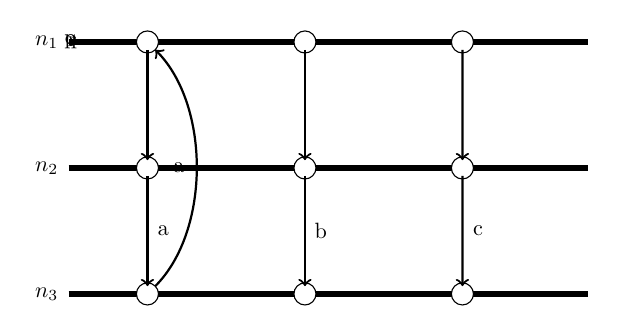
\begin{tikzpicture}[scale=0.8, every node/.style={transform shape}]

\begin{scope}[line width=2pt]
% Timelines for p, q, r and labels n1, n2, n3
\draw (-0.25, 0) -- (8, 0);
\draw (-0.25,-2) -- (8,-2);
\draw (-0.25,-4) -- (8,-4);
\end{scope}

% Line labels
\node[pos=0, left] at (-0.25, 0) {p};
\node[pos=0, left] at (-0.25,-2) {q};
\node[pos=0, left] at (-0.25,-4) {r};

% Node labels on timelines (n1, n2, n3)
\node at (-0.6,0) {$n_1$};
\node at (-0.6,-2) {$n_2$};
\node at (-0.6,-4) {$n_3$};

% Synchronized Nodes (white circles)
% Column A (action a)
\filldraw [fill=white] (1, 0) circle (1.75mm) node (pA) {};
\filldraw [fill=white] (1,-2) circle (1.75mm) node (qA) {};
\filldraw [fill=white] (1,-4) circle (1.75mm) node (rA) {};

% Column B (action b)
\filldraw [fill=white] (3.5, 0) circle (1.75mm) node (pB) {};
\filldraw [fill=white] (3.5,-2) circle (1.75mm) node (qB) {};
\filldraw [fill=white] (3.5,-4) circle (1.75mm) node (rB) {};

% Column C (action c)
\filldraw [fill=white] (6, 0) circle (1.75mm) node (pC) {};
\filldraw [fill=white] (6,-2) circle (1.75mm) node (qC) {};
\filldraw [fill=white] (6,-4) circle (1.75mm) node (rC) {};

\begin{scope}[thick,->]
% Downward chains for all columns
\draw (pA) -- (qA);
\draw (qA) -- (rA);
\draw (pB) -- (qB);
\draw (qB) -- (rB);
\draw (pC) -- (qC);
\draw (qC) -- (rC);

% Return loop for Column A (action a)
\draw (rA) .. controls (2,-3) and (2,-1) .. (pA);
\end{scope}

% Labels for actions (a, b, c) and return loop
\node at (1.25,-3) {a};
\node at (1.5,-2) {a}; % on return loop
\node at (3.75,-3) {b};
\node at (6.25,-3) {c};

\end{tikzpicture}
\caption{Three synchronized chains illustrating independent actions a, b, c on timelines p, q, r. The action 'a' features a time-disconnected recursive loop, leading to unbounded local time accumulation for agent r.}
\label{fig:synchronized-chains}
\end{figure}

An LTN $\Nn$ is \emph{weakly connectedly-communicating} if for every loop
$C = C_1 \xrightarrow{n_1} C_2 \xrightarrow{n_2} \cdots \xrightarrow{n_k} C_{k+1}=C$
in $\mg(\nuntime)$, letting $\Pi(C)=\{\pi_1,\dots,\pi_\ell\}$, the following holds:
for every block $\pi_i$, the communication graph of the loop restricted to vertices $\pi_i$
(i.e.\ edges induced by time-synchronizing nodes whose domains intersect $\pi_i$)
is connected.
\end{definition}

This condition is strictly weaker than Definition~\ref{def:connected-comm}:
it permits loops in which the full-agent communication graph is disconnected,
as long as every \emph{permanent synchronization class} remains internally connected.

\paragraph{Blockwise drift-boundedness.}
Since different blocks are, by construction, forever non-synchronizing with each other,
it is not meaningful to demand a uniform drift bound between agents in different blocks.
Instead, we require bounded drift \emph{within} each block.

\begin{definition}[Blockwise drift bound]
\label{def:blockwise-drift}
Let $(C,v)$ be a configuration and $\Pi(C)=\{\pi_1,\dots,\pi_\ell\}$.
We say $(C,v)$ is \emph{$k$-blockwise drift-bounded} if for every block $\pi_i$
and all $p,q\in \pi_i$ we have $|v(t_p)-v(t_q)|\le k$.
An LTN is \emph{$k$-blockwise drift-bounded} if every run can be tightened
to a run whose every configuration is $k$-blockwise drift-bounded.
\end{definition}

\paragraph{Why the proof technique still applies.}
The tightening construction (via slack graphs and back-edges between successive time-synchronizing events of the same agent) is agnostic to the global connectivity requirement: it operates on a given trace and preserves feasibility of guards and synchronizations.

The only place where connected communication was used essentially is in propagating bounds between arbitrary agents by chaining synchronizations across a loop.
In the weak setting, this propagation is performed \emph{within each block $\pi_i$ separately}:
over any sufficiently long segment that contains a loop, agents in a fixed block $\pi_i$
still form a connected communication graph, hence the same ``synchronization-chaining''
argument bounds the spread between the minimum and maximum timestamps \emph{inside $\pi_i$}.
Agents in different blocks are simply ignored, because no future synchronization constraints will ever relate their reference clocks.

\begin{theorem}[Weak connected communication implies blockwise bounded drift]
\label{thm:weak-cc-blockwise}
Every weakly connectedly-communicating LTN is $k$-blockwise drift-bounded for
\[
k \in O\!\left(|N|\cdot |A|^3 \cdot (M+1)\right),
\]
where $|N|$ is the number of nodes, $|A|$ the number of agents, and $M$ the maximum constant appearing in guards.
\end{theorem}

\begin{proof}[Proof sketch (adaptation)]
The proof follows the same template as for Theorem~\ref{thm:cc-bounded-drift}.
We tighten an arbitrary run to a tight run using the slack-graph construction.
Then we chunk the run into segments long enough to guarantee a repeated marking.

Fix a chunk starting at marking $C$ and consider the partition $\Pi(C)$.
For a block $\pi\in\Pi(C)$, restrict attention to the sub-trace induced by agents in $\pi$
and to time-synchronizing events whose domains intersect $\pi$.
By Definition~\ref{def:weak-cc}, every loop encountered inside the chunk induces a connected communication graph on $\pi$,
so the same chaining argument bounds the difference between the maximum and minimum timestamps attained by agents in $\pi$
within the chunk by a uniform function of $|N|,|A|,$ and $(M+1)$.
Since $\Pi(\cdot)$ only refines along the run, later chunks can only split blocks further,
which can only weaken the requirement (boundedness is required on smaller sets).
Stitching the bounds across chunks yields a uniform $k$ kfor all blocks throughout the run.
\end{proof}

\paragraph{Algorithmic and modelling consequences.}
This fragment strictly enlarges the applicability of the decidability result:
it admits systems where some agents permanently stop synchronizing with others
(e.g.\ an agent that continues to interact only through non-synchronizing nodes),
while still guaranteeing that within each permanent synchronization class,
clock drift can be bounded after tightening.
For the reachability decision procedure, the only additional bookkeeping is to track (or conservatively approximate) the current partition $\Pi(C)$ in the abstract state space and to enforce region-equivalence constraints \emph{per block} rather than globally.

\section{Conclusion}
\label{sec:conclusion}

We have developed a comprehensive theory of connectedly-communicating local-timed negotiations, proving that this fragment has decidable reachability via bounded drift.

\subsection{Summary of Contributions}

\begin{enumerate}
\item \textbf{Tightening algorithm} (Section~\ref{sec:tighten}): We formalized the notion of slack in distributed time-synchronizing systems through:
  \begin{itemize}
  \item Slack graphs that capture both available time reductions and synchronization constraints
  \item A tightening procedure that systematically reduces unnecessary delays
  \item The notion of tight traces as a normal form for behaviors
  \end{itemize}

\item \textbf{Bounded drift theorem} (Section~\ref{sec:cc-ltn-bounded}): We proved that connectedly-communicating LTNs have drift bounded by $\mathcal{O}(|N| \cdot |P|^3 \cdot (M+1))$ through:
  \begin{itemize}
  \item Chunking runs into segments containing complete marking-graph cycles
  \item Exploiting the connected communication graphs to propagate timing constraints
  \item Showing that tight runs have uniformly bounded timestamp differences
  \end{itemize}

\item \textbf{Decidability}: As a corollary, reachability is decidable for connectedly-communicating LTNs via region automaton construction on the set of tight untimed behaviors.
\end{enumerate}

\subsection{Future Directions}

\paragraph*{Efficient Verification}

While we have established decidability, the region automaton construction has well-known efficiency limitations. LTNs are attractive because they allow concurrency while restricting time-synchronizations to specific user-designated nodes. This suggests several research directions:

\begin{enumerate}
\item \textbf{Zone-based algorithms}: Can we develop partial-order reduction techniques that exploit the independence structure of LTNs, similar to what's been done for networks of timed automata?

\item \textbf{Compositional methods}: The modular structure of LTNs (multiple agents, multiple nodes) suggests compositional verification approaches. Can we verify properties of individual agents or sub-networks and compose the results?

\item \textbf{Symbolic methods}: BDD-based or SMT-based approaches might handle the bounded drift region space more efficiently than explicit enumeration.
\end{enumerate}

\paragraph*{Practical Applications}

LTNs model distributed systems where agents coordinate at specific points but otherwise act independently. Promising application domains include:

\begin{itemize}
\item \textbf{Cyber-physical systems}: Sensors that periodically synchronize with a central controller
\item \textbf{Distributed protocols}: Processes that occasionally synchronize via barriers or rendezvous
\item \textbf{Workflow systems}: Business processes with multiple parties that coordinate at specific milestones
\end{itemize}

Developing case studies in these domains would help validate the utility of the connectedly-communicating fragment and guide further theoretical development.

\paragraph*{Relaxing Connectedness}

Can we identify other syntactic restrictions beyond connectedness that ensure bounded drift? Some possibilities:

\begin{itemize}
\item Acyclic communication structures (no cyclic dependencies between synchronizations)
\item Bounded-depth hierarchies (limits on the ''distance'' between synchronizing agents)
\item Probabilistic or timed guarantees (synchronization occurs with sufficient frequency)
\end{itemize}

\paragraph*{Generalizations}

Our results assume discrete time and integer-valued constants. Extensions to dense time and multi-clock systems remain open. Additionally, combining LTNs with other formalisms (e.g., pushdown systems, probabilistic choice) could broaden applicability.

\subsection{Closing Remarks}

This work shows that local-timed negotiations admit a non-trivial decidable fragment through the lens of connectedness. The key insight---that connected communication graphs prevent unbounded drift---bridges ideas from distributed systems, timed automata, and controller synthesis.

The tightening framework we developed (Section~\ref{sec:tighten}) has independent interest as a general technique for analyzing distributed time-synchronizing systems. The slack graph construction and backward edge propagation might apply to other formalisms beyond LTNs.

More broadly, we hope this work motivates further study of LTNs as a sweet spot between expressiveness and tractability for modeling distributed real-time systems. The ability to selectively designate time-synchronizing points, combined with decidable verification, makes LTNs an attractive target for both theoretical investigation and practical application.